\documentclass[
  reprint,
  amsmath,
  amssymb,
  aps,
  pra,
  nofootinbib,
  superscriptaddress,
  floatfix
]{revtex4-2}
\usepackage[T1]{fontenc}
\usepackage{lmodern}
\usepackage{newunicodechar}
\newunicodechar{’}{'}
\usepackage{graphicx}
\graphicspath{{../../}{}}
\usepackage{capt-of} % \captionof for non-floating figures (used with widetext)
\usepackage{booktabs}
\usepackage{bm}
\usepackage{mathtools}
\usepackage{amsthm}
\usepackage{xcolor}
\usepackage{hyperref}
\hypersetup{hidelinks}

\newcommand{\placeholder}[1]{\textcolor{red!70!black}{\ifmmode\left[#1\right]\else\textsf{[#1]}\fi}}
\newcommand{\tentative}[1]{\textcolor{red!70!black}{#1}}
\newcommand{\structlabel}[1]{\noindent\mbox{\tentative{#1.}}~}
\newcommand{\Oset}{\mathcal{O}}
\newcommand{\Gset}{\mathcal{G}}
\newcommand{\Rset}{\mathcal{R}}
\newcommand{\Sset}{\mathcal{S}}
\newcommand{\Hcal}{\mathcal{H}}
\newcommand{\Bcal}{\mathcal{B}}
\newcommand{\Ocal}{\mathcal{O}}
\newcommand{\Ucal}{\mathcal{U}}
\newcommand{\Jcal}{\mathcal{J}}
\newcommand{\Pcal}{\mathcal{P}}
\newcommand{\Dcal}{\mathcal{D}}
\newcommand{\Wcal}{\mathcal{W}}
\newcommand{\dd}{\mathrm{d}}
\newcommand{\ii}{\mathrm{i}}
\newcommand{\ee}{\mathrm{e}}
\newcommand{\TR}{\mathrm{TR}}
\newcommand{\ex}{\mathrm{ex}}
\newcommand{\ctrl}{\mathrm{ctrl}}
\newcommand{\stat}{\mathrm{stat}}
\newcommand{\dyn}{\mathrm{dyn}}
\newcommand{\drv}{\mathrm{drv}}
\newcommand{\obs}{\mathrm{obs}}
\newcommand{\stay}{\mathrm{stay}}
\newcommand{\app}{\mathrm{append}}
\newcommand{\ablate}{\mathrm{ablate}}
\newcommand{\Var}{\operatorname{Var}}
\newcommand{\Tr}{\operatorname{Tr}}
\newcommand{\Top}{\operatorname{Top}}
\newcommand{\argminp}{\mathop{\mathrm{arg\,min}}}
\newcommand{\argmaxp}{\mathop{\mathrm{arg\,max}}}
\newcommand{\proj}{\mathrm{proj}}
\newcommand{\diag}{\mathrm{diag}}
\newcommand{\CVaR}{\operatorname{CVaR}}
\newcommand{\softmax}{\operatorname{softmax}}
\newcommand{\hh}{\mathrm{HH}}
\newcommand{\phmax}{n_{\mathrm{ph,max}}}
\newcommand{\twq}{\mathrm{2Q}}
\newcommand{\eps}{\varepsilon}
\newcommand{\ket}[1]{|#1\rangle}
\newcommand{\bra}[1]{\langle #1|}
\newcommand{\braket}[2]{\langle #1|#2\rangle}
\newcommand{\expval}[1]{\langle #1\rangle}
\newcommand{\metrichead}[1]{\makebox[0.061\textwidth][c]{#1}}
\newcommand{\archmetrichead}[1]{\makebox[0.040\textwidth][c]{#1}}
\newcommand{\inlinetablecaption}[2]{%
  \par\addvspace{1.6ex}%
  \captionof{table}{#2\label{#1}}%
  \par\addvspace{0.8ex}%
}
\newenvironment{schurlemma}[1][]
{\par\medskip\noindent\textbf{Lemma}\if\relax\detokenize{#1}\relax\else\ (#1)\fi.\space\itshape}
{\par\medskip}
\newenvironment{schurassumption}[1][]
{\par\medskip\noindent\textbf{Assumption}\if\relax\detokenize{#1}\relax\else\ (#1)\fi.\space}
{\par\medskip}
\newenvironment{schurtheorem}[1][]
{\par\medskip\noindent\textbf{Theorem}\if\relax\detokenize{#1}\relax\else\ (#1)\fi.\space\itshape}
{\par\medskip}
\newenvironment{schurremark}[1][]
{\par\medskip\noindent\textbf{Remark}\if\relax\detokenize{#1}\relax\else\ (#1)\fi.\space}
{\par\medskip}


\begin{document}

\makeatletter
\def\bibsection{\section*{\refname}\@nobreaktrue}
\makeatother

\title{Geometric and Resource-Aware Adaptive Ansatz Construction Applied to the Hubbard--Holstein Dimer}

\author{Jake Strobel}
\author{Jacopo Simoni}
\author{Gabriele Riva}
\author{Yuan Ping}
\affiliation{University of Wisconsin--Madison}

\date{\today}

% PROVENANCE(EDITORIAL_FRAMING_NOTES_20260718) archived -> MATH/paper_facing/paper_I_static_scaffold/provenance/Paper_I_inline_comment_archive_20260727.md
\begin{abstract}
Near-term ground-state quantum simulation requires adaptive ansätze that
achieve high accuracy while limiting circuit depth and quantum-estimator
overhead. ADAPT-VQE constructs ansätze by iteratively selecting generators
from an operator pool using first-order energy derivatives. Consequently, its
standard selection rule does not model directional curvature, the relaxation
of the active ansatz following candidate admission, or generator-specific
circuit and measurement costs. We introduce Resource-Aware ADAPT (RA-ADAPT),
whose central contribution is a four-phase selection procedure, Phases 0--III,
that progressively enriches the generator score from the standard ADAPT
gradient to local response models evaluated once about the fixed optimized
source state at each outer-loop iteration. The procedure progressively
escalates local response modeling before ranking candidates by predicted energy
decrease after local active-ansatz relaxation per resource cost. Its final phase uses a Schur-reduced quadratic
trust-region model of the joint candidate and active-ansatz response in the
Fubini--Study pullback metric. The response solve is restricted to the retained
metric support, while accepted refits use a fixed pullback-whitened chart that
excludes Gram-null parameter directions and orthonormalizes the retained
Fubini--Study tangents for coordinate-sensitive inner optimization.
Lowerre-style beam continuation, Tetris-style batch admission, and generator
ablation arise as natural extensions of this same energy-per-resource model.
We evaluate plateau-triggered RA-ADAPT on the two-site Hubbard--Holstein model
using the same symmetry-retained single-Pauli-word operator pool as
Append-ADAPT across six interaction regimes. At a common attainable accuracy
before the earlier effective plateau, RA-ADAPT requires less logical estimator
work in five regimes and fewer routed two-qubit gates in four. Within a shared
logical-estimator budget, RA-ADAPT reaches a lower same-cutoff energy error in
all six regimes, with at least a tenfold reduction in five. The accepted
trajectories further identify spin-resolved intersite electronic hopping as
the dominant descent channel and show that stronger Holstein coupling
increases the contribution from mixed electron--phonon channels at weak and
intermediate Hubbard interaction.


\end{abstract}

\maketitle







\section{Introduction}

Quantum processing units (QPUs) promise computational speedups for classically hard problems, including the simulation of quantum many-body physics \cite{Lloyd1996,AspuruGuzik2005}. A central task is preparing the ground state of a given Hamiltonian. The scope of available simulation problems is limited by QPU resource constraints, including circuit depth, entangling-gate count, and measurement overhead \cite{Preskill2018NISQ,Cerezo2021VQA,Huggins2021Measurements}. This current QPU regime is classified as the noisy intermediate-scale quantum (NISQ) era, and many classes of algorithms have been developed specifically to address these bottlenecks. One such class is adaptive derivative-assembled pseudo-Trotter variational quantum eigensolvers (ADAPT-VQE), which iteratively construct circuits by appending gates from a predefined operator pool according to an energy-gradient selection rule. ADAPT-VQE has been developed primarily for small fermionic systems \cite{Anastasiou2024,Bespalova2026KADAPT,He2026HAADAPT,He2026ParamADAPT}, with recent extensions to vibrational Hamiltonians and bosonic lattice models \cite{Majland2024vADAPT,Athanasakos2026CVADAPT}. It can nevertheless fail to reach the desired ground-state accuracy because of prohibitive circuit depths and measurement overhead, insufficiently expressive operator pools, or energy plateaus arising from poorly conditioned variational-coordinate landscapes \cite{Grimsley2019,Tang2021,Yordanov2021,Feniou2023,Ramoa2025HessianRecycling,Ikhtiarudin2025ShotEfficient,Stadelmann2025GradientTroughs}. Thus ansatz construction through operator selection becomes the dominant lever for NISQ ground-state preparation. We present Resource-Aware ADAPT as a highly accurate, resource-aware operator-selection subroutine of ADAPT-VQE. For brevity, we refer to Resource-Aware ADAPT as Resource-ADAPT (RA).


\subsection{Modeled problem}
Previous quantum-algorithm studies of electron--phonon systems have largely focused on qubit encodings, variational basis compression, hybrid quantum--classical solvers, and simulation frameworks \cite{Macridin2018,Li2023,Denner2023,Peng2025BosonHamiltonians}. By contrast, a standard ADAPT-VQE construction framework for condensed-matter fermion--phonon Hamiltonians, including the Hubbard--Holstein model, has not yet emerged. This gap is particularly relevant because electronic-structure applications of ADAPT-VQE can rely on a mature hierarchy of unitary coupled cluster singles and doubles excitation operators, such as UCCSD \cite{Romero2018UCC,Grimsley2019}, whereas mixed fermion--phonon condensed-matter models require operator pools that simultaneously represent electronic correlation, lattice excitations, and electron--phonon dressing. Operator-pool design therefore becomes part of the algorithmic problem. For the Hubbard--Holstein model, the pool must contain generators that capture electronic correlation, phononic lattice response, and coupled electron--phonon dressing. After encoding, these mixed-sector generators require gates that entangle fermionic and bosonic registers under a finite phonon-mode truncation \cite{Hubbard1963,Holstein1959a,Holstein1959b}. The Hubbard--Holstein operator pool is defined in Appendix~\ref{app:hh_operator_pool}. We study six interaction-strength regimes and compare RA-ADAPT against append-only ADAPT-VQE through same-cutoff energy errors, transpiled circuit resources, and estimator queries at matched attained accuracy and at the selected terminal horizons.


The Hubbard--Holstein model \cite{ClayHardikar2005HH,Tezuka2007HH} is written as
\begin{align}
H
&=-t\sum_{\langle i,j\rangle,\sigma}
(c_{i\sigma}^{\dagger}c_{j\sigma}+c_{j\sigma}^{\dagger}c_{i\sigma})
+U\sum_i n_{i\uparrow}n_{i\downarrow}
\nonumber\\
&\quad+\omega_0\sum_i b_i^\dagger b_i
+g\sum_i(b_i^\dagger+b_i)(n_i-\bar n).
\label{eq:hubbard_holstein_static}
\end{align}
Here \(c_{i\sigma}\) and \(b_i\) are the fermionic and bosonic annihilation operators on site \(i\); their Hermitian conjugates (\(\dagger\)) are the corresponding creation operators; \(\sigma \in\{\uparrow, \downarrow\}\) denotes particle spin;
\(n_{i\sigma}, n_i\) are the spin-resolved and total fermionic number operators, respectively; \(\bar n=N_e/L\) is the mean fermion filling for fixed electron number \(N_e\) and lattice size \(L\). Our results use open boundary conditions with half-filling. Here \(t\) is the nearest-neighbor electronic hopping amplitude, \(U\) is the onsite Hubbard interaction, \(\omega_0\) is the phonon frequency, \(g\) is the local electron--phonon coupling, and \(\langle i,j\rangle\) denotes nearest-neighbor lattice sites.
In the joint decoupling limit $g\to0$ and $\omega_0\to0$, the electronic sector reduces to the Hubbard Hamiltonian, up to a decoupled zero-frequency phonon register. We use Jordan--Wigner and binary encoding for Eq.~\eqref{eq:hubbard_holstein_static} and the operator-pool generators in Appendix~\ref{app:hh_operator_pool}, with fixed blocked qubit registers \cite{Sawaya2020,Peng2025BosonHamiltonians}.


\subsection{Current status}
ADAPT-VQE constructs a parameterized circuit iteratively by adding operators from a predefined pool according to an energy-gradient criterion \cite{Grimsley2019,Tang2021,Yordanov2021}.
At each outer-loop iteration, the algorithm evaluates candidate generators and selects one whose infinitesimal insertion produces the largest-magnitude first-order energy response. For the mixed fermion--boson system considered here, the reference state is a Hartree--Fock Slater determinant tensored with the phonon vacuum at a chosen mode cutoff,
\begin{equation*}
\ket{\psi_{\mathrm{ref}}}=\ket{\mathrm{HF}}\otimes\ket{0_1\,0_2\,\cdots\,0_M}.
\end{equation*}
Here \(M\) is the number of retained phonon modes. Given an encoded Hamiltonian \(H\), an operator pool \(\mathcal G\), and the reference state \(\ket{\psi_{\mathrm{ref}}}\), append-only ADAPT-VQE adds one selected generator at each outer-loop iteration. If \(U_k(\boldsymbol{\theta}_k)\) is the current ansatz, its update is
\begin{equation*}
U_{k+1}(\boldsymbol{\theta}_{k},\alpha)
=e^{-i\alpha A_k^\star}U_k(\boldsymbol{\theta}_{k}).
% source label: eq:adapt_append_update
\end{equation*}
Here \(\boldsymbol{\theta}_k\) is the active parameter vector, \(A_k^\star\in\mathcal G\) is the selected Hermitian generator, and \(\alpha\) is its zero-amplitude trial coordinate. The selected generator satisfies
\begin{equation}
A_k^\star\in\operatorname*{arg\,max}_{A\in\mathcal G}
\left|
\left.
\partial_{\alpha}E\!\left(e^{-i\alpha A}U_k(\boldsymbol{\theta}_{k}^\star)\ket{\psi_{\mathrm{ref}}}\right)
\right|_{\alpha=0}
\right|\,,
\label{eq:adapt_append_gradient}
\end{equation}
where \(E\) is the Hamiltonian expectation value of the indicated trial state. Here and below, a superscript \(\star\) marks a selected or optimized extremizer. After each outer-loop insertion, a classical optimizer refits the active parameters according to the Rayleigh--Ritz criterion \cite{Peruzzo2014,McClean2016,Kandala2017}:
\begin{equation}
\label{eq:theta_opt}
\boldsymbol{\theta}^\star
=\arg\min_{\boldsymbol{\theta}}
\bra{\psi_{\rm ref}}U^\dagger(\boldsymbol{\theta})HU(\boldsymbol{\theta})
\ket{\psi_{\rm ref}}\,.
\end{equation}
Numerous ADAPT variants modify the outer-loop generator-selection rule. CEO-ADAPT combines related qubit excitations acting on the same spin-orbital set into coupled-exchange generators \cite{Ramoa2025}. Overlap-ADAPT incorporates tangent-direction information into the append criterion \cite{Feniou2023}. Other methods exploit second-order derivative information to improve convergence \cite{Grimsley2023ADAPT} or recycle Hessian information to reduce the cost of repeated inner-loop optimizations \cite{Ramoa2025HessianRecycling}. Contemporaneous with this work, Geo-ADAPT-VQE applies the inverse of the full-pool tangent Gram matrix to the energy-gradient covector and appends the generator associated with the largest-magnitude component of the resulting collective tangent direction; Pos-Geo-ADAPT extends this geometric rule from append-only selection to generator insertion \cite{Sohail2026GeoADAPT}. Prune ADAPT addresses circuit growth by removing previously selected generators using amplitude- and history-based criteria \cite{Vaquero2025PrunedADAPT}.

\subsection{Limitations with current approaches}
Despite these advances, current adaptive strategies leave several issues unresolved. Standard ADAPT selects generators using first-order energy gradients \cite{Grimsley2019,Tang2021,Yordanov2021}. This local criterion can be myopic: a generator with the largest instantaneous gradient need not produce the largest energy decrease after the ansatz parameters are reoptimized, and it may lead to deeper circuits than curvature-aware selection rules \cite{Feniou2023,Grimsley2023ADAPT}. Existing selection algorithms also do not explicitly estimate the candidate-specific energy gain produced by the combined response of the new generator and the variational parameters. In addition, without an explicit resource penalty, two candidates with similar gradient or energy-gain estimates can be treated as nearly equivalent even when they differ substantially in two-qubit gate count, routing depth, or measurement cost.
Geo-ADAPT incorporates state-space geometry by solving a full-pool inverse-Gram problem and selecting the generator associated with the largest-magnitude component of the resulting collective tangent direction \cite{Sohail2026GeoADAPT}. However, constructing the full Gram matrix scales as $\mathcal{O}(|\mathcal{G}|^2)$, and the inverse problem may become ill-conditioned when the pool contains redundant or nearly redundant tangent directions \cite{Sohail2026GeoADAPT,Ramoa2025HessianRecycling,Ikhtiarudin2025ShotEfficient}.
% PROVENANCE(PRESERVED_GEO_ADAPT_DESCRIPTION_20260726) archived -> MATH/paper_facing/paper_I_static_scaffold/provenance/Paper_I_inline_comment_archive_20260727.md

These limitations motivate a candidate-specific joint second-order response model, symmetric resource-cost weighting, and staged screening that reserves the most expensive response evaluations for the most competitive candidates.




%
\subsection{\textsc{RA-ADAPT}: geometric and resource-aware ansatz growth}
At each outer-loop iteration, \textsc{RA-ADAPT} fixes the current optimized
ansatz as the source state and applies a four-phase candidate-selection
procedure before admitting and refitting a proposal. Phase 0 ranks the complete
executable candidate population by the standard ADAPT absolute energy
gradient and retains a fixed prefix without Fubini--Study metric evaluation or
resource-cost weighting. Phase I applies a first-order trust-region screen,
Phase II adds one-dimensional candidate curvature while holding the active
ansatz fixed, and Phase III evaluates the surviving records with a
second-order response model that jointly optimizes the candidate amplitude and
active-ansatz relaxation within a Fubini--Study trust region
\cite{Nocedal2006TrustRegion,ProvostVallee1980,Stokes2020QNG,Haug2021Capacity,VanStraaten2021MeasurementCost}.
The resulting Phase-III model estimates the energy decrease available after
local active-ansatz relaxation. The phase scores progress from the standard
absolute gradient in Phase 0 to predicted energy decrease per symmetric
relative resource cost in Phases I--III. The same cost construction is used
in Phases I--III. Phase I supplies its circuit coordinates from a
fixed hardware-graph estimate; in the compiled-cost configuration, Phases II
and III evaluate those same coordinates by Qiskit transpilation. The reported
undecomposed-generator proxy-only diagnostic retains the graph estimates
through Phases I--III.
The predicted Phase-III joint displacement calibrates the trust radius after
refit. After admission,
retained-support whitening is applied separately to condition the accepted
inner refit.

The resource penalty combines circuit and measurement costs. Its circuit
coordinates are two-qubit count, two-qubit depth, and one-qubit work, evaluated
either by the fixed-graph construction or by transpilation as just described.
The parameter and measurement coordinates are unchanged by that choice.
Measurement cost is estimated from grouped Pauli measurements and the
additional shot demand required to estimate the candidate-gradient observable
\cite{Verteletskyi2020CliqueCover,Yen2020CompatibleMeasurements,Ikhtiarudin2025ShotEfficient}.
Thus candidates with similar predicted energy gains can be distinguished by
the hardware and measurement resources required to realize and score them.

\textsc{RA-ADAPT} can also admit more than one candidate in a single outer-loop update. The highest-ranked records are tested for tangent nonredundancy and predicted additive energy descent after variational refit. A compatible set may then be admitted jointly; we refer to this operation as batching.

Among the score-ordered proposals, \textsc{RA-ADAPT} may instantiate leading
individual-record or batch proposals as parallel circuit branches using a
Lowerre-style beam search \cite{Lowerre1976Beam}. Each branch is refitted
independently, and branch retention is
determined by realized energy gain per added circuit cost.


To reduce unnecessary circuit growth, \textsc{RA-ADAPT} permits ablation of existing generators whose variational directions have become locally redundant. The same second-order local Taylor--Schur model with a regularized Fubini--Study metric predicts whether the surviving ansatz can recover the pre-ablation state and energy after a generator is removed. The deletion is retained when the refitted energy loss is small relative to the corresponding circuit-cost reduction \cite{Vaquero2025PrunedADAPT}; otherwise the original ansatz is restored and the generator is placed on cool-down.

\textsc{RA-ADAPT} uses plateau-triggered insertion to open internal ansatz positions when append-only growth ceases to produce a prescribed energy decrease. The selector then ranks generator--position records by predicted energy improvement and relative resource cost. Append-only and always-insertion selection are the limiting cases in which the internal-position domain is held closed or open, respectively, at every outer iteration.
% PROVENANCE(FUTURE_INSERTION_DIAGNOSTIC_20260724) archived -> MATH/paper_facing/paper_I_static_scaffold/provenance/Paper_I_inline_comment_archive_20260727.md

Across Phases 0--III, the staged restriction limits the measurement overhead
of higher-order response scoring by reducing the candidate population before
each more expensive phase. Phase 0 scouts generator identities at
the append endpoint using only standard ADAPT gradients. The retained
identities are then expanded over the active insertion-position domain before
Phase I. Quantities are carried forward when the candidate representation is
unchanged. In the reported comparisons, the executable representation is
fixed before Phase 0: one route screens intact operator-pool generators, and
the other screens the complete symmetry- and padding-valid single-Pauli-word
pool. The selected executable pool remains fixed throughout Phases 0--III.
Appendix~\ref{app:pauli_word_pool} defines the single-Pauli-word pool
construction. The resulting procedure retains the top-scored records before the
next, more expensive phase is evaluated; see
Fig.~\ref{fig:static_adapt_selector_flow}.

\section{Staged generator-position ranking}
\label{sec:static_method}
%
\begin{figure*}[t]
\centering
\setlength{\fboxsep}{6pt}
\resizebox{0.97\textwidth}{!}{%
\begin{tabular}{c@{\;\(\longrightarrow\)\;}c@{\;\(\longrightarrow\)\;}c@{\;\(\longrightarrow\)\;}c@{\;\(\longrightarrow\)\;}c@{\;\(\longrightarrow\)\;}c}
\fbox{\parbox[c][3.7cm][c]{2.3cm}{\centering
\textbf{Executable pool}\\[2mm]
intact generators or guarded Pauli words}} &
\fbox{\parbox[c][3.7cm][c]{2.4cm}{\centering
\textbf{Phase 0}\\
standard ADAPT screen\\[2mm]
\(\Delta E_0(r)=\lvert g(r)\rvert\)\\[2mm]
retain top \(N_0\)}} &
\fbox{\parbox[c][3.7cm][c]{2.4cm}{\centering
\textbf{Phase I}\\
first-order screen\\[2mm]
\(S^{(1)}=\Delta E_1/K_1\)\\[1mm]
graph-evaluated circuit coordinates\\[2mm]
retain top \(N_1\) globally}} &
\fbox{\parbox[c][3.7cm][c]{2.4cm}{\centering
\textbf{Phase II}\\
directional-curvature screen\\[2mm]
\(S^{(2)}=\Delta E_2/K_2\)\\[1mm]
transpiled circuit coordinates\\[2mm]
retain top \(N_2\) globally}} &
\fbox{\parbox[c][3.7cm][c]{2.4cm}{\centering
\textbf{Phase III}\\
candidate--active response\\[2mm]
\(S^{(3)}=\Delta E_3/K_3\)\\[1mm]
transpiled circuit coordinates\\[2mm]
rank remaining records}} &
\fbox{\parbox[c][3.7cm][c]{2.2cm}{\centering
\textbf{Admit and refit}\\[2mm]
insert selected record at its recorded position\\[2mm]
full-ansatz reoptimization}}
\end{tabular}%
}
\caption{RA-ADAPT staged candidate-selection flow across Phases 0--III.
Phase 0 retains generator identities by the unweighted standard ADAPT absolute
gradient, Phase I applies the cost-aware first-order screen, Phase II applies
the second-order directional model, and Phase III reranks the remaining
records through the Schur-reduced candidate--active response. The relative-cost
construction in Phases I--III uses fixed-graph circuit coordinates in Phase I,
whereas the compiled-cost configuration evaluates those coordinates by
Qiskit transpilation in Phases II and III. The proxy-only diagnostic
instead retains the graph evaluation through Phase III.
The selected record is inserted at
its recorded position before full-ansatz reoptimization.}
\label{fig:static_adapt_selector_flow}
\end{figure*}

At outer iteration \(k\), the optimized source ansatz is held fixed while
Phases 0--III execute one staged selection procedure. Each phase
restricts the population before the next, more expensive response model is
evaluated. For records whose representation is unchanged, later phases augment
the measurements acquired on the larger earlier population and reuse the
Phase-II compiled-cost cache in Phase III. The shared active-coordinate Gram
and Hessian blocks are acquired once per outer iteration.

RA-ADAPT inserts operators within the ordered generator unitary
\(U(\boldsymbol{\theta})\) through the plateau-triggered position policy. The insertion domain remains append-only
until an accepted full refit produces an energy decrease below a prescribed
opening threshold; the next selection round then opens
the full commutation-reduced domain. Before scoring, positions
separated only by active generators certified to commute with the candidate
are collapsed to one deterministic representative. This quotient removes
unitary-equivalent insertion orderings and prevents equivalent
candidate--position records from being scored and charged separately. The
domain is recomputed after every accepted refit and closes when the realized
decrease again reaches the threshold. Appendix~\ref{app:numerical_conventions}
gives the complete construction.

For \(A\in\mathcal G\), let \(\mathcal P_k(A)\) denote its admissible positions
at outer iteration \(k\). A candidate generator--position record is
\[
r=(A,p),
\]
with \(p\in\mathcal P_k(A)\), and the candidate record set is
\begin{equation}
\mathcal R_k
=
\bigcup_{A\in\mathcal G}
\{A\}\times\mathcal P_k(A).
\label{record_set}
\end{equation}
The outer-loop index \(k\) remains fixed throughout the selection procedure, so we suppress
it from the phase-indexed record sets. Let \(\mathcal R^{(t)}\) be the
population evaluated in Phase \(t\), for \(t\in\{0,1,2,3\}\). Phase 0 ranks
\(\mathcal R^{(0)}\) at the append endpoint, retains the \(N_0\) largest
gradient magnitudes, and expands those generator identities over the active
position domain to form \(\mathcal R^{(1)}\).
Phase I restricts \(\mathcal R^{(1)}\) to \(\mathcal R^{(2)}\), Phase II restricts
\(\mathcal R^{(2)}\) to \(\mathcal R^{(3)}\), and Phase III ranks
\(\mathcal R^{(3)}\) by its joint candidate--active response. The Phase-0
score is \(S^{(0)}(r)=\Delta E_0(r)=|g(r)|\). In Phases I--III, each record
\(r\in\mathcal R^{(t)}\) receives
\(S^{(t)}(r)=\Delta E_t(r)/K_t(r)\), where \(\Delta E_t(r)\) is the
phase-dependent predicted energy drop and \(K_t(r)\) is the record's
population-relative resource-cost factor; see
Sec.~\ref{subsec:cost_weighted_record_ranking}.

The Phase-I restriction retains the highest-scoring records under the global
cap \(N_1\). Candidate identities remain unchanged between Phases I and II.
Appendix~\ref{app:record_restriction} gives the restriction maps.

The remaining task is to define the predicted energy decrease \(\Delta E(r)\) and relative resource-cost factor \(K(r)\) that determine the phase score.

\section{Candidate scoring}
\subsection{Phase-dependent energy models}
\label{subsec:candidate_energy_models}
%
Phases 0--III use progressively richer energy models. Phase 0 uses the standard
ADAPT gradient magnitude, Phase I applies a first-order trust-region model,
Phase II adds candidate-direction curvature, and Phase III evaluates records
\(r\in\mathcal R^{(3)}\) with a local quadratic model that couples the
candidate coordinate to the active ansatz. We present these nested models from
Phase III to Phase 0.
\paragraph*{Coupled local quadratic model.}
%
Let \(\alpha\) denote the candidate coordinate of the compiled generator
\(A\mapsto e^{-i\alpha A}\), and let \(\delta\boldsymbol{\theta}\) denote a
displacement of the active ansatz coordinates from the optimized source point
\(\boldsymbol{\theta}_k^\star\) of \(U_k\). For each candidate record \(r=(A,p)\), let
\(E_r(\alpha,\delta\boldsymbol{\theta})\) denote the exact energy surface of
the candidate-augmented ordered ansatz about this source point.
The Phase-III model is the second-order expansion of this surface about
\((\alpha,\delta\boldsymbol{\theta})=(0,\mathbf 0)\):
\begin{equation}
E_r(\alpha,\delta\boldsymbol{\theta})
\approx
E_0
+ g_{\alpha}\alpha
+ \frac{1}{2}H_{\alpha\alpha}\alpha^2
+ \alpha H_{\alpha\boldsymbol\theta}\delta\boldsymbol{\theta}
+ \frac{1}{2}\delta\boldsymbol{\theta}^{\top}
H_{\boldsymbol\theta\boldsymbol\theta}\delta\boldsymbol{\theta},
\label{eq:local_quadratic}
\end{equation}
where \(E_0=E(U_k(\boldsymbol\theta_k^\star))\) and the active-coordinate first
derivatives are set identically to zero under the stationary-source model. They
are therefore neither acquired nor charged to Phase III. The scalar \(g_\alpha\)
is the signed candidate-direction derivative,
and the four Hessian blocks $H_{uv}$ describe
candidate curvature ($\alpha\alpha$), candidate--ansatz coupling
($\alpha\boldsymbol\theta$), and active-ansatz response
($\boldsymbol\theta\boldsymbol\theta$).

We use Eq.~(\ref{eq:local_quadratic}) to score records by comparing their predicted energy drop. In compact form, the predicted energy difference given by Eq.~\eqref{eq:local_quadratic} is
\begin{equation}
\Delta E(\mathbf z)
=
\mathbf g^\top \mathbf z
+
\frac{1}{2}\mathbf z^\top \mathbf H\mathbf z,
\label{eq:compact_local_quadratic}
\end{equation}
where the joint coordinate displacement and gradient are
\begin{equation}
\mathbf z
=
\begin{pmatrix}
\alpha\\
\delta\boldsymbol{\theta}
\end{pmatrix},
\qquad
\mathbf g
=
\begin{pmatrix}
g_\alpha\\
\mathbf 0
\end{pmatrix}.
\end{equation}
The Hessian has the block structure
\begin{equation}
\mathbf H
=
\begin{pmatrix}
H_{\alpha\alpha} & H_{\alpha\boldsymbol\theta}\\
H_{\boldsymbol\theta\alpha} &
H_{\boldsymbol\theta\boldsymbol\theta}
\end{pmatrix}, \qquad
H_{uv}:=\left.\partial_u\partial_vE_r\right|_{(0,\mathbf 0)}
\label{eq:hessian_block_def}
\end{equation}
where \(u,v\in\{\alpha,1,\ldots,|\boldsymbol{\theta}|\}\). We restrict the
predicted displacement to a local region defined by the Fubini--Study metric
\(\mathbf G\):

\begin{equation}
\mathbf z^\top \mathbf G\mathbf z
\le
\rho^2,
\label{eq:fs_trust_region}
\end{equation}
where \(\rho\) is the trust radius, calibrated after admission by comparing
predicted and realized motion in the same source-point metric. The
Fubini--Study metric is then given by
\[
\mathbf G
=
\begin{pmatrix}
G_{\alpha\alpha} & G_{\alpha\boldsymbol\theta}\\
G_{\boldsymbol\theta\alpha} &
G_{\boldsymbol\theta\boldsymbol\theta}
\end{pmatrix}, \qquad G_{uv}:=\Re\!\left[\left.\langle \partial_u\psi \middle| \Pi \middle| \partial_v\psi\rangle\right|_0\right]
\]

where $\Pi=\mathbb I - \ket{\psi}\bra{\psi}$ projects onto the subspace
orthogonal to \(\ket{\psi}\). This removes the nonphysical global-phase
direction so that the metric measures physical first-order changes of the
quantum state.

\paragraph*{Phase III predicted energy drop.}
On the retained tangent support, the numerical procedure returns the
generalized trust-region minimizer \(\mathbf z_3^\star(r)\) satisfying
\(\bigl[\mathbf z_3^\star(r)\bigr]^\top
\mathbf G\mathbf z_3^\star(r)\le\rho^2\).
The unshifted quadratic model assigns this step the predicted decrease
\begin{equation}
\Delta E_3(r)
=-g(r)\alpha_3^\star(r)
-\frac12\bigl[\mathbf z_3^\star(r)\bigr]^\top
\mathbf H\mathbf z_3^\star(r) .
\label{eq:phase3_model}
\end{equation}
The retained-support stationarity equations Schur-eliminate the active-ansatz
response \(\delta\boldsymbol\theta\).
Appendix~\ref{app:numerical_conventions} specifies the trust-region multiplier,
complementarity condition, and supported pseudoinverse used to obtain
\(\mathbf z_3^\star(r)\). The resulting
joint displacement is scored by Eq.~\eqref{eq:phase3_model}, and its predicted
energy decrease determines generator admission through the relative resource
cost of \(r\) defined below.

The local Taylor--Schur model extends directly to optional batch admission and
generator ablation. For a batch \(B\), the scalar candidate coordinate \(\alpha\) is
replaced by the block
\(\boldsymbol\alpha_B=(\alpha_r)_{r\in B}\), which is optimized jointly with
the active-ansatz response \(\delta\boldsymbol\theta\) within the supported
Phase-III trust region. For deletion at ansatz position \(p\), the candidate
displacement is fixed to \(\alpha=-\theta_p^\star\), while the surviving
coordinates \(\delta\boldsymbol\theta_{\setminus p}\) minimize the
metric-regularized Schur surrogate; after accepted deletion,
the ansatz is parameterized by \(\boldsymbol\theta_{\setminus p}\). The
batch-compatibility and delete--refit validation rules are given in
Appendices~\ref{app:batching} and~\ref{app:optional_structure_management}.

\paragraph*{Phase II predicted energy drop.}
Phase II assumes no coupling between \(\alpha\) and
\(\delta\boldsymbol{\theta}\). Setting
\(\delta\boldsymbol\theta=\mathbf 0\) in
Eq.~\eqref{eq:local_quadratic} removes the candidate--ansatz response blocks.
Its one-dimensional predicted decrease is
\begin{equation}
\Delta E_2(r)=
\max_{\alpha^2G_{\alpha\alpha}\le\rho^2}
\left[
-g(r)\alpha
-\frac12H_{\alpha\alpha}\alpha^2
\right].
\label{eq:phase2_gain}
\end{equation}

\paragraph*{Phase I predicted energy drop.}
Phase I further omits directional curvature. Its predicted decrease is
\begin{equation}
\Delta E_1(r)
=\max_{\alpha^2G_{\alpha\alpha}\le\rho^2}[-g(r)\alpha]
=\frac{\rho\,|g(r)|}{\sqrt{G_{\alpha\alpha}}}.
\label{eq:phase1_gain}
\end{equation}

\paragraph*{Phase 0 gradient screen.}
Phase 0 uses the standard ADAPT gradient magnitude as its predicted decrease:
\begin{equation}
\Delta E_0(r)=\lvert g(r)\rvert.
\label{eq:phase0_gain}
\end{equation}

Appendix~\ref{app:numerical_conventions} gives the Phase-II optimizer and its
scalar degenerate cases.

\paragraph*{Observable evaluation.}
%
The energy and geometric models use the following circuit-measurable quantities.
For a candidate record \(r=(A,p)\), factor the optimized source circuit at
\(p\) into the partial circuits \(U_{k,>p}\) and \(U_{k,\le p}\), and define
the exact candidate-augmented family
\begin{align*}
U_r(\alpha,\delta\boldsymbol{\theta})
&:=
U_{k,>p}\!\left(
\boldsymbol{\theta}_{k,>p}^{\star}
+\delta\boldsymbol{\theta}_{>p}
\right)
e^{-i\alpha A}\\[-0.2em]
&\phantom{{}:={}}\;
U_{k,\le p}\!\left(
\boldsymbol{\theta}_{k,\le p}^{\star}
+\delta\boldsymbol{\theta}_{\le p}
\right),\\
U_r(0,\mathbf 0)
&=U_k(\boldsymbol{\theta}_k^\star).
\end{align*}
Let
\(\ket{\psi_r(\alpha,\delta\boldsymbol\theta)}
:=U_r(\alpha,\delta\boldsymbol\theta)\ket{\psi_{\rm ref}}\), so that
\(E_r(\alpha,\delta\boldsymbol\theta)
=\bra{\psi_r(\alpha,\delta\boldsymbol\theta)}
H\ket{\psi_r(\alpha,\delta\boldsymbol\theta)}\).
The gradient of $\ket{\psi}$ with respect to a generator's amplitude coordinate $u$ evaluated over $u=0$ gives
\(\left.\partial_u\ket{\psi}\right|_0=-i\widetilde A_u\ket{\psi}\), where
\(\widetilde A_r=U_{k,>p}AU_{k,>p}^{\dagger}\).
For any observable \(O\), expectation values over the current ansatz are denoted by
\begin{equation*}
\langle O\rangle:=\langle\psi|O|\psi\rangle.
\end{equation*}
The signed candidate derivative is therefore the measurable commutator
expectation
\begin{equation}
g(r)=g_\alpha
=i\left\langle[\widetilde A_r,H]\right\rangle.
\label{eq:record_gradient}
\end{equation}

The exact ordered-coordinate energy Hessian is
\begin{equation}
H_{uv}
=
2\operatorname{Re}\!\left[
\left\langle
\partial_u\partial_v\psi_r
\middle|H\middle|\psi
\right\rangle
+
\left\langle
\partial_u\psi_r
\middle|H\middle|
\partial_v\psi_r
\right\rangle
\right]_{(0,\mathbf0)} .
\label{eq:joint_hessian_observable}
\end{equation}
This expression includes the coordinate dependence of the dressed generators
induced by the ordered product circuit.

The projected Fubini--Study Gram-matrix entries are
\begin{equation}
\begin{aligned}
G_{uv}
&=\frac12\left\langle
\{\widetilde A_u,\widetilde A_v\}
\right\rangle
-\left\langle\widetilde A_u\right\rangle
 \left\langle\widetilde A_v\right\rangle .
\end{aligned}
\label{eq:joint_gram_observable}
\end{equation}

\subsection{Relative resource-cost factor}
\label{subsec:cost_weighted_record_ranking}
%
The phase score is the predicted energy decrease per relative resource cost:
\begin{equation}
S^{(t)}(r)
=
\frac{\Delta E_t(r)}{K_t(r)}\,.
\label{eq:master_phase_score}
\end{equation}
Here \(\Delta E_t(r)\) is the phase-\(t\) predicted energy decrease defined in
Sec.~\ref{subsec:candidate_energy_models}, and \(K_t(r)>0\) is the
phase-dependent relative cost factor defined below.

To distinguish below-median from above-median resource burden, \textsc{RA-ADAPT}
divides each phase gain by the dimensionless relative resource-cost factor
\(K_t(r)\). For each record, this factor combines two-qubit count,
two-qubit depth, one-qubit work, added parameter dimension, and
grouped-measurement shot demand. The cost factor has the same form in every
phase; only the evaluation of the three circuit coordinates changes. Phase I
uses the fixed hardware-graph construction defined below. In the compiled-cost
configuration, Phases II and III evaluate these same circuit coordinates after
Qiskit transpilation. The parameter and measurement coordinates retain the
definitions below. In the reported single-generator comparisons,
\(\widehat C_\theta=1\) for every record, so population centering removes this
coordinate from the ranking. The grouped-measurement shot coordinate is also
uniform within each scored single-Pauli-word population. It remains
candidate-dependent for intact generators because their Pauli-polynomial
contents differ. The proxy-only configuration uses the graph evaluation in all
three phases.

For a system of \(Q\) qubits, fix a candidate record \(r=(A,p)\). The associated compiled generator is expressed as a Pauli polynomial,

\begin{equation}
A=\sum_{\mu}c_{\mu}P_{\mu}, \qquad P_{\mu}\in\{I,X,Y,Z\}^{\otimes Q}\,.
\label{eq:pauli_expansion}
\end{equation}
%
Here \(\mu\) indexes the nonzero terms in the expansion, and \(c_\mu\) is the
coefficient of the Pauli word \(P_\mu\).
For each such Pauli word, we define its qubit support as
%
\begin{equation}
\begin{aligned}
S_{\mu}
&:=\operatorname{supp}(P_{\mu}) \\
&=\{q\in\{1,\ldots,Q\}:(P_{\mu})_q\ne I\}.
\end{aligned}
\label{eq:pauli_word_support}
\end{equation}
%
The Phase-I graph estimates below are computed from these Pauli-word supports. Larger supports require longer parity-computation circuits, while supports spread across the hardware graph require larger entangling depth or routing overhead. For a Pauli exponential compiled by a CNOT ladder, a multi-qubit Pauli rotation is implemented by reducing it to a single-qubit rotation with additional entangling gates. A Pauli word acting on \(s=|S_{\mu}|\) qubits requires \(s-1\) \textsc{CNOT}s before the \(R_z\) rotation and \(s-1\) \textsc{CNOT}s after it to restore the original qubit register. The CNOT count is estimated by
%
\begin{equation*}
\widehat C_{\mathrm{CX}}(r)=\sum_{\mu}2\,\max[|S_{\mu}|-1, 0],
% source label: eq:pauli_2count_proxy
\end{equation*}
whereas the layout-aware two-qubit depth is given by
\begin{equation*}
\widehat C_d(r)=\sum_{\mu}2\,\operatorname{span}_{G}
\bigl(S_{\mu}\bigr)\,.
% source label: eq:pauli_2depth_proxy
\end{equation*}
Here \(G\) is the hardware connectivity graph, and $\operatorname{span}_{G}(S_{\mu})$ is the number of edges in the shortest connected subgraph containing the support \(S_{\mu}\). The quantity is set to zero when $|S_{\mu}|\le1$. This term penalizes Pauli words whose active qubits are far apart in the connected graph.

The same Pauli-rotation circuit also uses one-qubit basis-change gates. Let
\[
S_{\mu}^{XY} = \{q\in S_{\mu}:(P_{\mu})_q = X\text{ or }Y\}
\]
On each qubit in \(S_{\mu}^{XY}\), we rotate into the \(Z\) basis before the Pauli rotation and rotate it back afterward. Let \(c_q(g)\) denote the contribution of a one-qubit gate \(g\) on qubit \(q\) to this basis-change cost proxy. If the required basis rotation is $V_{\mu q}$, its forward and back cost is
\[
c_q^{\pm}(V_{\mu q})=c_q(V_{\mu q})+c_q(V^{-1}_{\mu q})\,.
\]
The one-qubit cost of this Pauli word is then given by
%
\begin{equation*}
\widehat{C}_{1q,\mu}(r) = \sum_{q\in S_{\mu}^{XY}}c_q^\pm(V_{\mu q}) + c_{\bar{q}_{\mu}}(R_z)\,.
\end{equation*}
Here \(\bar{q}_{\mu}\) is the qubit where the central rotation \(R_z\) is applied. The total one-qubit cost then becomes \(\widehat{C}_{1q}(r)=\sum_\mu\widehat{C}_{1q,\mu}(r)\). The parameter cost is the number of new independent parameters added by candidate \(r\):
\begin{equation*}
\widehat C_\theta(r)
=
|\boldsymbol\vartheta_r|.
% source label: eq:parameter_cost_proxy
\end{equation*}
%
Here \(\boldsymbol\vartheta_r\) is the parameter block introduced by record
\(r\). For single-generator insertion this is one; batched or tied insertions
may add a different number of independent parameters. The measurement cost is
computed from the candidate-gradient commutator
\(i[\widetilde A_r,H]\)
\cite{Verteletskyi2020CliqueCover,Yen2020CompatibleMeasurements}, which after
qubit mapping is rewritten as a sum of Pauli words
%
\[
i[\widetilde A_r,H]=\sum_{\nu=1}^{N_r}c_{r\nu}P_{r\nu}\,.
\]
%
Here \(N_r\) is the number of Pauli words in the mapped candidate-gradient operator, \(c_{r\nu}\) are Pauli coefficients, and \(P_{r\nu}\) are Pauli words.
The Pauli words are then grouped into qubit-wise commuting blocks, denoted by
\(\Pi_r\), so that all Pauli words in the same block can be measured using a
single basis. The marginal shot estimate accounts for measurement bases
already acquired during earlier scoring phases. Let
\(C_r\subseteq\Pi_r\) contain the blocks compatible with those cached bases.
These blocks have zero additional basis cost, so only the blocks in
\(\Pi_r\setminus C_r\) require new measurement bases.
For each new block \(C\), we assign the coefficient weight
\[
w_C = \sqrt{\sum_{\nu\in C}|c_{r\nu}|^2}\,.
\]
The shot-cost proxy is then given by
\begin{equation*}
\widehat C_{\rm shot}(r)=
\frac{1}{\sigma_\star^2}
\left[
\sum_{C\in\Pi_r\setminus C_r}
w_C
\right]^2\,.
% source label: eq:shot_cost_proxy
\end{equation*}
%
Here $\sigma_\star$ is the target standard error for the candidate-gradient estimate \cite{Ikhtiarudin2025ShotEfficient}. This proxy gives a lower cost to candidates whose gradient reuses existing measurement bases and a higher cost to candidates that require new measurement blocks with large Pauli coefficients.

For cost component
\(x\in\{\mathrm{CX},d,1q,\theta,\mathrm{shot}\}\), define the
phase-\(t\) median, median-absolute-deviation scale, and signed cost coordinate
over the records being scored by \cite{IglewiczHoaglin1993}
\begin{equation}
\begin{aligned}
m_x(t)
&:=
\operatorname*{median}_{r'\in\mathcal R^{(t)}}
\widehat C_x(r'),\\
s_x(t)
&:=
\operatorname*{median}_{r'\in\mathcal R^{(t)}}
\left|\widehat C_x(r')-m_x(t)\right|,\\
\bar C_x(r;t)
&:=
\frac{2}{\pi}
\arctan\!\left(
\frac{\widehat C_x(r)-m_x(t)}{s_x(t)}
\right).
\end{aligned}
\label{eq:cost_robust_excess}
\end{equation}
Thus \(\bar C_x(r;t)\in[-1,1]\), with negative values for below-median costs
and positive values for above-median costs. The bounded arctangent transform
compresses large deviations while preserving their sign. For nonnegative
weights with \(\sum_x\lambda_x>0\), the phase-\(t\)
relative resource-cost factor is
\begin{equation}
K_t(r)
=
\left[
1-\frac{1}{2}
\frac{
\displaystyle\sum_x\lambda_x\bar C_x(r;t)
}{
\displaystyle\sum_x\lambda_x
}
\right]^{-1}
\in\left[\frac{2}{3},2\right].
\label{eq:hardware_cost_sum}
\end{equation}
%
The weights \(\lambda_{\mathrm{CX}}\), \(\lambda_d\), \(\lambda_{1q}\),
\(\lambda_\theta\), and \(\lambda_{\rm shot}\) set the relative importance of
the CNOT-count, layout-aware-depth, one-qubit, parameter, and shot-cost
coordinates. Below-median records receive \(K_t(r)<1\), whereas above-median
records receive \(K_t(r)>1\).

\section{Ansatz admission and refit}
\label{subsec:ansatz_admission_refit}
\paragraph*{Admission and whitened refit.}
%
The Phase-III records are evaluated with
Eq.~\eqref{eq:phase3_model} and ranked by \(S^{(3)}\). For individual-record
admission, the returned record satisfies
\begin{equation*}
r_k^\star
\in
\operatorname*{arg\,max}_{r\in\mathcal R^{(3)}}S^{(3)}(r).
\end{equation*}
Its generator is inserted at its recorded position, and the enlarged ansatz is
fully reoptimized under Eq.~\eqref{eq:theta_opt} with the new amplitude
initialized to zero or warm-started at the Phase-III candidate-amplitude
optimum \(\alpha_3^\star(r)\) used in Eq.~\eqref{eq:phase3_model}. When beam
search is enabled, the leading records instead instantiate separate child
branches that are refitted independently.
Optional batch admission is defined in Appendix~\ref{app:batching}.

\paragraph*{Retained Phase-III tangent support.}
%
To define the retained tangent support, a symmetric eigensolver supplies
eigenpairs \(\mathbf G\mathbf v_i=\lambda_i\mathbf v_i\). Let \(V\) collect
the eigenvectors satisfying
\begin{equation}
\lambda_i>\eta\max_j\lambda_j.
\label{eq:phase3_support_threshold}
\end{equation}
where \(\eta\) is the relative rank tolerance. The Phase-III optimization in
Eq.~\eqref{eq:phase3_model} is performed over the retained tangent support
\(\operatorname{range}(V)\), so
\(\mathbf z\in\operatorname{range}(V)\). The retained Gram eigenvalues
preserve their original scaling in the Fubini--Study trust metric.

\paragraph*{Accepted-refit whitening.}
For the proposal admitted after Phase III---either a singleton record or a
batch satisfying the conditions in Appendix~\ref{app:batching}---the accepted
ansatz is assigned the inherited zero-insertion base point
\(\boldsymbol\theta^{(0)}\), which retains the optimized iteration-\(k\)
logical amplitudes and places each newly admitted generator at the insertion
position specified by its record with zero amplitude. The inner refit is
initialized either at this base point or warm-started by setting the new
amplitudes to the corresponding candidate components of the Phase-III optimum
used in Eq.~\eqref{eq:phase3_model}, or of its batch extension in
Appendix~\ref{app:batching}. In what follows, we specialize to one logical
circuit amplitude per generator.
Thus
\(\boldsymbol\theta\in
\mathbb R^{\lvert\boldsymbol\theta^{(0)}\rvert}\)
denotes a generic inner-optimization iterate. Consequently,
\[
\ket{\psi_{k+1}(\boldsymbol\theta^{(0)})}
=
\ket{\psi_k(\boldsymbol\theta_k^\star)}.
\]

Let \(\mathbf G^{(0)}\) be the Fubini--Study Gram matrix of the accepted
ansatz \(\ket{\psi_{k+1}(\boldsymbol\theta)}\), evaluated at
\(\boldsymbol\theta^{(0)}\). This source-point matrix is the accepted
Phase-III joint Gram matrix whose row and column indices are permuted from
response-coordinate order into post-admission circuit-parameter order and
reused without additional estimator acquisition. Circuit-coordinate
displacements are identified modulo
\(\ker\mathbf G^{(0)}\), so the physical first-order directions are
represented by the quotient
\begin{equation}
\mathbb R^{\lvert\boldsymbol\theta^{(0)}\rvert}
\big/
\ker\mathbf G^{(0)}.
\label{eq:accepted_refit_quotient}
\end{equation}
The form induced by \(\mathbf G^{(0)}\) descends to a positive-definite
Fubini--Study inner product on this quotient, whose circuit-coordinate
representatives generally retain local anisotropy.

After quotienting the exact Gram-null directions,
Eq.~\eqref{eq:phase3_support_threshold} further restricts the quotient to its
numerically resolved support. Let \(V\) collect the retained eigenvectors of
\(\mathbf G^{(0)}\), evaluated with \(\mathbf G=\mathbf G^{(0)}\), and let
\(\Lambda\) contain the corresponding eigenvalues:
\[
\mathbf G^{(0)}V=V\Lambda.
\]
The inverse square root is formed on these retained positive modes, whose
image may be a proper subspace of the exact quotient. Define
\begin{equation}
W=V\Lambda^{-1/2},
\qquad
W^{\top}\mathbf G^{(0)}W=I.
\label{eq:accepted_refit_whitening}
\end{equation}
The equivalence classes of the columns of \(W\) form a Fubini--Study
orthonormal basis of the retained quotient support, and their projected state
derivatives form the corresponding orthonormal tangent frame. Let
\(\mathbf y\in\mathbb R^{\operatorname{rank}(V)}\) denote a coordinate vector
in this frame. Hence
\[
\mathbf y
\longmapsto
W\mathbf y+\ker\mathbf G^{(0)}
\]
is an isometric isomorphism onto the retained quotient support. The fixed
matrix \(W\) is therefore a local preconditioner from tangent-frame
coordinates \(\mathbf y\) to logical circuit-coordinate displacements. The
inner optimizer uses the affine parameterization
\[
\boldsymbol\theta(\mathbf y)
=
\boldsymbol\theta^{(0)}+W\mathbf y,
\]
begins at \(\mathbf y=\mathbf0\) for zero initialization or at the coordinates
of the Phase-III warm start, and returns \(\mathbf y^\star\), giving
\begin{equation}
\boldsymbol\theta_{k+1}^{\star}
=
\boldsymbol\theta^{(0)}+W\mathbf y^\star.
\label{eq:accepted_refit_endpoint}
\end{equation}
The frozen matrix \(W\) defines the orthonormal tangent frame at
\(\boldsymbol\theta^{(0)}\); the current Fubini--Study metric may vary during
the inner refit. A multiparameter extension replaces the scalar generator
coordinate by a parameter block and applies the same support restriction,
whitening, and refit in the enlarged coordinate space.

\paragraph*{Trust-radius update.}
The radius \(\rho_k\) defines the Fubini--Study trust domain shared by all
three scoring phases: Eq.~\eqref{eq:fs_trust_region} gives the joint Phase-III
domain, and Eqs.~\eqref{eq:phase2_gain} and~\eqref{eq:phase1_gain} give its
Phase-II and Phase-I restrictions. After the proposal is refitted, the next
iteration's radius is updated by comparing predicted and realized parameter
motion in the retained source-point Gram metric. Let
\(\delta\boldsymbol\theta^{\mathrm{pred}}\) be the Phase-III joint step
embedded in the enlarged ansatz coordinates, and let
\(\delta\boldsymbol\theta^{\mathrm{real}}
=\boldsymbol\theta_{k+1}^{\star}
-\boldsymbol\theta^{(0)}\). Using this source-point metric, define the
displacement
\begin{equation}
\left\|\delta\boldsymbol\theta\right\|_{\mathbf G^{(0)}}
=
\sqrt{
\delta\boldsymbol\theta^\top
\mathbf G^{(0)}
\delta\boldsymbol\theta
}.
\label{eq:source_metric_displacements}
\end{equation}
All quantities inside the outer brackets below are evaluated at iteration \(k\).
The update multiplies the current scalar radius by the square root of the
predicted-to-realized source-metric displacement ratio:
\begin{equation}
\rho_{k+1}
=
\left[
\rho
\times
\left[
\frac{
\left\|\delta\boldsymbol\theta^{\mathrm{pred}}\right\|_{\mathbf G^{(0)}}
}{
\left\|\delta\boldsymbol\theta^{\mathrm{real}}\right\|_{\mathbf G^{(0)}}
}
\right]^{1/2}
\right]_k .
\label{eq:adaptive_trust_radius}
\end{equation}
Thus larger-than-predicted motion contracts the radius, whereas
smaller-than-predicted motion expands it, subject to the numerical safeguards
and expansion convention in Appendix~\ref{app:numerical_conventions}. This
calibration reuses the source Gram information from the accepted refit and
requires no endpoint-overlap evaluation or additional quantum-query charge.

After this branch-local trust update, optional generator ablation may remove
one eligible ansatz entry \(d^\star\) under the acceptance rule in
Appendix~\ref{app:optional_structure_management}. Optional beam retention is
then applied to the refitted and, when enabled, ablated children. For a
retained branch with an accepted ablation, the ansatz update is
%
\begin{equation*}
U_{k+1}(\boldsymbol\theta_{k+1})
=
U_k(\boldsymbol\theta_k)
\oplus
r_k^\star
\ominus
d^\star .
% source label: eq:snake_ansatz_update
\end{equation*}
%
The symbol \(\oplus\) denotes admission of selected generator records into the
ordered ansatz, and \(\ominus\) denotes removal of that ansatz entry. When no
ablation is accepted, the final removal is omitted. The resulting branch state
is denoted \(\ket{\psi_{k+1}}\).

\paragraph*{Stopping condition.}
The natural stopping condition is an iteration-energy plateau: the realized
energy improvement after each accepted full refit remains below a prescribed
threshold for a fixed patience period.

The complete branchwise pseudocode is given in
Appendix~\ref{app:complete_algorithm}.

%\end{comment}


\section{Results}
\label{sec:results}
\label{sec:benchmarks}

We compare plateau-triggered RA-ADAPT and Append-ADAPT VQE on an equally
parameterized two-site Hubbard--Holstein model. Both methods use the same
symmetry-retained single-Pauli-word operator pool, encoding, reference state,
and inner-optimization protocol. Every pool element carries one variational
parameter.

The reported Hubbard--Holstein comparisons use half filling, open boundary conditions, and the same inner-optimization method for RA-ADAPT and append-only ADAPT within each candidate representation. The generator pool is defined in Appendix~\ref{app:hh_operator_pool}.

We report the same-cutoff absolute energy error
\(\lvert\Delta E_k(M)\rvert=\lvert E_k(M)-E_{\rm ED}(M)\rvert\)
\cite{Weisse2008}; weak- and
strong-Holstein sectors use local phonon cutoffs \(M=3\) and \(M=7\),
respectively, exactly filling two- and three-qubit binary registers.
% PROVENANCE(DEMOTED_HH_ED_CUTOFF_SPOT_CHECK_20260811):
% The available M<=10 scan is retained as diagnostic evidence rather than a
% reader-facing convergence claim because it does not establish truncation
% convergence below the smallest reported variational errors (~1e-14 |t|).
% Historical spot check across U/t in {0.25,1.25,8}: the M=3 weak-Holstein and
% M=7 strong-Holstein ED references differed from M=10 by at most 5.45e-7 |t|
% and 7.17e-8 |t|, respectively; the largest M=9-to-M=10 drift was 2.42e-10 |t|.
% Promotion requires regime-resolved cutoff sequences continued until successive
% ED energies are stable below 1e-14 |t|, with stability confirmed across more
% than one successive cutoff increment.
% Six-regime ED cutoff receipt:
% MATH/paper_facing/paper_I_static_scaffold/paper_i_hh_ed_cutoff_reference_six_regime_20260727.json
% sha256=66a6409790affffd6ce8928d7fb46cc945b57d50e210d3cb215e8039a63c5573
For each regime, the shared comparison window ends at the earlier effective
plateau, defined as the first iteration within \(10\%\) of a method's best
error. The common target \(\lvert\Delta E_\cap\rvert\) is the larger of the
two within-window minima, and each method is costed at its first crossing. A
second comparison fixes the logical-estimator budget at RA-ADAPT's expenditure
at its effective plateau, capped by the available Append-ADAPT expenditure,
and reports the best error reached by each method within that budget. The
iteration-\(50\) comparison is retained as a common-horizon endpoint check.

Circuit resources are the two-qubit gate count \(N_{2q}\), two-qubit depth
\(D_{2q}\), and total circuit depth \(D_c\) at the selected prefix. Each full circuit, including reference-state
preparation, is transpiled to the 156-qubit FakeMarrakesh target with native
basis \(\{\mathtt{sx},\mathtt{rz},\mathtt{x},\mathtt{cz},\mathtt{id}\}\),
optimization level \(1\), and seed \(7\)
\cite{JavadiAbhari2024Qiskit,QiskitAlgorithmsAdaptVQE}. Thus \(N_{2q}\)
includes routed \(\mathtt{cz}\) gates and SWAP overhead. The logical-estimator
quantity \(S_{\rm alg}\) is accumulated through the same prefix under the
closed occurrence convention of Appendix~\ref{app:estimator_queries}.


\subsection{Hubbard--Holstein benchmarks}
Using the parameterization convention given in Eq.~\eqref{eq:hubbard_holstein_static}, we report the interaction regimes in terms of \(U\), \(t\), \(g\), and \(\omega_0\).
For the Hubbard sector, we classify weak, intermediate, and strong electronic-correlation regimes using the dimer convention:

\begin{equation}
    U/t \in\{0.25,1.25,8\} \label{hubbard_regimes}
\end{equation}

Within each Hubbard correlation regime, we consider weak and strong Holstein electron--phonon coupling regimes. Using the Holstein dimer convention, \(\lambda=2g^2/(t\omega_0)\). We choose \(\omega_0/t=1\), which gives \(g/t=\sqrt{\lambda/2}\) \cite{Sakkinen2015HolsteinDimer}.
The chosen weak and strong Holstein coupling regimes are given by:

\begin{equation}
    \lambda\in\{0.25,1.25\} \label{holstein_sectors}
\end{equation}

These correspond to \(g/t=\sqrt{\lambda/2}=0.354\) and \(0.791\) in Eq.~\eqref{eq:hubbard_holstein_static}. Together these choices define six combined Hubbard--Holstein interaction regimes, obtained by crossing three Hubbard correlation regimes with two Holstein electron--phonon coupling regimes. The Cartesian product of Eqs.~\eqref{hubbard_regimes} and~\eqref{holstein_sectors} is used below for matched comparisons of RA-ADAPT and append-only ADAPT.


Results reported below use SciPy Powell with a maximum iteration budget of 200
for the inner optimization procedure of Eq.~\eqref{eq:theta_opt}. The displayed
trajectories span 50 ADAPT iterations for both methods.

The executable Phase-0 population contains 948 and 6508 globally guarded
single Pauli words for the weak- and strong-Holstein cutoffs, respectively.
Phase 0 retains the 24 largest standard-ADAPT gradient magnitudes. Phase I
rescores those 24 candidates and retains at most 24, Phase II evaluates that
population and retains at most 12, and Phase III ranks the remaining at most
12 records before admitting one. All restrictions use one global population.
The single-Pauli-word identities are constructed and symmetry filtered before
selection, then preserved throughout Phases 0--III.
The nonzero scalar coefficient is absorbed into the candidate coordinate,
\begin{equation*}
e^{-i\alpha c_\mu P_\mu}
=e^{-i\beta_\mu P_\mu},
\qquad
\beta_\mu:=\alpha c_\mu,
\end{equation*}
and the executed singleton uses the canonical unit Pauli representative \(P_\mu\).
This convention removes coefficient-induced rescaling from the conventional
Append-ADAPT gradient selector. The RA-ADAPT gains \(\Delta E_t\) are
invariant under any nonzero linear rescaling of the candidate coordinate.
The reported RA-ADAPT trajectories use no cost weighting in Phase 0. The
relative resource-cost factor is applied in Phases I--III. For the
single-Pauli-word route, Phase I uses the fixed-graph structural proxy, while
Phases II and III evaluate the same circuit-cost coordinates by Qiskit
transpilation; the Phase-III population reuses the Phase-II compilation cache
for unchanged records. The undecomposed-generator
proxy-only diagnostic uses the fixed-graph structural coordinates in Phases I--III.

% PROVENANCE(PHASE0_AND_COST_FIDELITY_20260811): standard-gradient Phase-0
% semantics and estimator scope are implemented in
% pipelines/static_adapt/ra_adapt/phase0.py. The Paper-I execution contracts
% use N0=24, N1=24, N2=12, and one-record admission. The reported global-
% singleton route uses fixed-graph Phase-I and Qiskit-evaluated
% Phase-II/III costs; the reported macro proxy-only diagnostic uses fixed-graph
% structural costs in Phases I--III. Executable-pool counts are
% resolved per cutoff from the representation adapters in
% pipelines/static_adapt/ra_adapt/adapters.py and their locked run protocols.

% PROVENANCE(MACHINE_READABLE_PAPER_I_SNAKE_CANONICAL_SETTINGS_GUARD_20260709) archived -> MATH/paper_facing/paper_I_static_scaffold/provenance/Paper_I_inline_comment_archive_20260727.md

% PROVENANCE(MACHINE_READABLE_HH_PHYSICAL_LANE_DUPLICATE_UPDATE_20260708) archived -> MATH/paper_facing/paper_I_static_scaffold/provenance/Paper_I_inline_comment_archive_20260727.md
%
% PROVENANCE(MACHINE_READABLE_PAPER_I_S_ACCOUNTING_CORRECTION_20260709) archived -> MATH/paper_facing/paper_I_static_scaffold/provenance/Paper_I_inline_comment_archive_20260727.md
%
% PROVENANCE(MACHINE_READABLE_PAPER_I_HH_ITERATION50_INSERTION_RESULTS_20260727) archived -> MATH/paper_facing/paper_I_static_scaffold/provenance/Paper_I_inline_comment_archive_20260727.md
%
% COMPONENT_EVIDENCE_UPDATE(20260731): the main overlays use the evolving
% stationary-core page-1/page-2 trajectories. The report is cross-revision
% partial progress, so the numerical summaries are not yet final paper evidence.
% Receipt: MATH/paper_facing/paper_I_static_scaffold/provenance/
% paper_i_append_stationary_core_v6_component_adoption_20260729.json
% sha256=36b692255e73dd8287de5e309259e1f8703dd0ef4e2f5e889279e97c2c4d23ce
% Macro overlay provenance is the page-1 stationary-source matched-error
% candidate generated by build_paper_i_hh_insertion_policy_overlays.py.
% Macro overlay provenance sha256=99336586e4c6625b45440c9c15b406b58154b9c43291fca2e851c5221fcb3af1
% Singleton overlay provenance sha256=a3d3a3da40a338b44d6f73ff65f1a8b924f73f9f736109f6a80fa147c5282fb9
% COMPONENT_EVIDENCE_UPDATE(20260813): the main-text figure and compact table
% use the plateau-triggered projected-singleton matched comparison in
% output/pdf/paper_i_ra_vs_append_matched_comparisons_20260812.pdf.
% Reader-facing figure generated by
% pipelines/reporting/clean_paper_i_ra_append_singleton_matched_plot.py.
% COMPONENT_EVIDENCE_UPDATE(SINGLETON_POLICY_COMPARISON_20260814): the weak-
% Holstein panels use six authenticated k=50 comparator trajectories, and the
% weak--strong panel additionally uses its authenticated append-only trajectory,
% trajectories in output/pdf/paper_i_ra_adapt_stationary_core_full48_r50_20260728_evolving/
% paper_i_ra_adapt_stationary_core_full48_r50_20260728_evolving_page12_singleton_insertion_comparator_snapshot_adapter.json.
% The new policy curves carry terminal markers only; the open-circle and
% triangle markers remain reserved for the primary plateau-insertion versus
% Append-ADAPT matched comparison.
% COMPONENT_EVIDENCE_UPDATE(STRONG_HOLSTEIN_POLICY_COMPARISON_20260815):
% the terminally passed local k=50 always-insertion trajectory for weak--strong,
% together with always-insertion and append-only trajectories for
% intermediate--strong and strong--strong, comes from
% output/local_runs/paper_i_page12_strong_holstein_sector5_local_repair_20260814_v1/.
% Exact terminal, manifest, guard, worker-receipt, and summary hashes are
% recorded in the v8 figure
% provenance JSON beside the generated figure.
\clearpage
\onecolumngrid
\noindent\begin{minipage}{\textwidth}
\begin{center}
\includegraphics[width=0.98\textwidth]{figures/paper_i_ra_vs_append_matched_singleton_plateau_20260812/paper_i_ra_vs_append_matched_singleton_plateau.pdf}
\captionof{figure}{RA-ADAPT and Append-ADAPT VQE using the same
symmetry-retained single-Pauli-word pool. Each panel shows the same-cutoff
energy error through iteration \(50\). All six panels additionally show
RA-ADAPT with insertion active throughout and RA-ADAPT restricted to the
append endpoint.
Diamonds and squares mark the corresponding terminal values. Open circles
mark the first common-accuracy crossings for the primary plateau-triggered
RA-ADAPT versus Append-ADAPT comparison, and filled triangles mark the best
errors within the shared \(S_{\rm alg}\) budget.}
\label{fig:hh_singleton_matched_plateau}
\end{center}
\end{minipage}
\clearpage
\twocolumngrid
\par\addvspace{0.45ex}
\begin{table}[t]
\caption{\label{tab:hh_singleton_matched_plateau}
First-crossing costs at the shared same-cutoff error
\(\lvert\Delta E_\cap\rvert\) for plateau-triggered RA-ADAPT and
Append-ADAPT. Circuit costs are reported as
\(C_{\rm circ}=(N_{2q},D_{2q},D_c)\) at the listed ADAPT iteration
\(k_\cap\).}
\centering
\footnotesize
\setlength{\tabcolsep}{2.2pt}
\renewcommand{\arraystretch}{1.02}
\begin{tabular}{@{}llrrl@{}}
\toprule
Regime & Method & \(k_\cap\) & \(C_{\rm circ}\) & \(S_{\rm alg}\) \\
\midrule
W--W \((1\mathrm{e}{-9})\) & RA & 37 & \((371,285,865)\) & \(1.1\mathrm{e}5\) \\
     & Ap & 37 & \((402,323,990)\) & \(2.8\mathrm{e}5\) \\
\addlinespace[0.25ex]
I--W \((6\mathrm{e}{-9})\) & RA & 34 & \((375,297,898)\) & \(9.8\mathrm{e}4\) \\
     & Ap & 32 & \((347,259,777)\) & \(3.0\mathrm{e}5\) \\
\addlinespace[0.25ex]
S--W \((1\mathrm{e}{-6})\) & RA & 11 & \((83,63,198)\) & \(1.7\mathrm{e}4\) \\
     & Ap & 11 & \((50,46,159)\) & \(1.6\mathrm{e}4\) \\
\addlinespace[0.25ex]
W--S \((6\mathrm{e}{-4})\) & RA & 35 & \((306,218,691)\) & \(3.0\mathrm{e}5\) \\
     & Ap & 50 & \((597,449,1371)\) & \(1.2\mathrm{e}6\) \\
\addlinespace[0.25ex]
I--S \((1\mathrm{e}{-4})\) & RA & 39 & \((330,264,863)\) & \(3.4\mathrm{e}5\) \\
     & Ap & 49 & \((510,383,1146)\) & \(1.2\mathrm{e}6\) \\
\addlinespace[0.25ex]
S--S \((3\mathrm{e}{-8})\) & RA & 45 & \((479,388,1204)\) & \(4.3\mathrm{e}5\) \\
     & Ap & 45 & \((519,389,1127)\) & \(9.2\mathrm{e}5\) \\
\bottomrule
\end{tabular}
\end{table}

At the common accuracy target, plateau-triggered RA-ADAPT reduces
\(S_{\rm alg}\) in five regimes, by factors from \(2.13\) to \(3.80\), and
reduces \(N_{2q}\) in four. Weak--weak, weak--strong, and
intermediate--strong reduce every reported circuit coordinate together with
the estimator count. Intermediate--weak exchanges an \(8\%\) increase in
\(N_{2q}\) for a \(3.07\)-fold reduction in estimator work. The
strong--weak crossing occurs at the same iteration for both methods and favors
Append-ADAPT in circuit and estimator resources.

At common \(S_{\rm alg}\), plateau-triggered RA-ADAPT reaches the lower error
in every regime. The reduction exceeds one order of magnitude in five:
\(7.57\times10^5\) in weak--weak, \(7.41\times10^7\) in
intermediate--weak, \(15.1\) in weak--strong, \(19.1\) in
intermediate--strong, and \(10.2\) in strong--strong. Strong--weak reaches
essentially the same error for both methods. At iteration \(50\), RA-ADAPT has
the lower error in weak--weak, intermediate--weak, weak--strong, and
intermediate--strong, while Append-ADAPT has the lower endpoint error in the
two strong-Hubbard regimes. The matched comparisons in
Table~\ref{tab:hh_singleton_matched_plateau} provide the resource-normalized
comparison.

The weak-Holstein policy trajectories isolate the role of positional search.
In weak--weak, insertion active throughout and plateau-triggered insertion
both reach the \(10^{-15}\) error scale at iteration \(50\). The RA-ADAPT
append endpoint and conventional Append-ADAPT end at the \(10^{-9}\) scale.
In intermediate--weak, the two insertion routes reach the
\(10^{-14}\)--\(10^{-15}\) scale, and the two append routes end at the
\(10^{-9}\) scale. In strong--weak, the three RA-ADAPT insertion policies end
near \(1.4\times10^{-6}\), and conventional Append-ADAPT reaches
\(8.0\times10^{-7}\). Positional freedom therefore changes the attainable
accuracy in the weak- and intermediate-Hubbard sectors of the weak-Holstein
row. The strong-Hubbard sector retains the same \(10^{-6}\) terminal scale
across the three RA-ADAPT insertion policies.
% PROVENANCE(MACHINE_READABLE_PAPER_I_RA_APPEND_SINGLETON_SUPPORT_SHARE_20260811):
% receipt=MATH/paper_facing/paper_I_static_scaffold/provenance/paper_i_ra_append_singleton_support_share_prose_20260811.json
% sha256=0304c1b6e3fb9f9c4f3ba172bc4dc9dacd22adb93c7e8ea212a6e24f4b0ec293
% builder=pipelines/reporting/build_paper_i_ra_append_singleton_support_share_evidence.py
% regenerate=python3 pipelines/reporting/build_paper_i_ra_append_singleton_support_share_evidence.py
% metric=p_{S,r}^{(m)}=100*sum_{k:supp(P_k)=S}max(0,E_{k-1}-E_k)/sum_k max(0,E_{k-1}-E_k)
% normalization=independent within each method--regime pair at k=50; displayed values rounded to 0.1 percentage point
% semantics=path-dependent realized accepted-step descent; not a causal ablation or connected-correlation observable
% adoption=user-directed Paper-I Results adoption of the authenticated Append-ADAPT k=1:50 prefixes on 2026-08-11

The accepted single-Pauli-word trajectories reveal which physical response
channels carry the realized variational descent.  In the blocked register, the
first two qubits represent the spin-up electronic orbitals on the first and
second lattice sites, and the next two represent the corresponding spin-down
orbitals.  The final four qubits form two binary phonon registers, with one
two-qubit register assigned to each lattice site.  This ordering identifies
whether a selected word represents intersite electronic motion, a local
electron--phonon response, a cross-site electron--phonon response, or a purely
phononic response.  For each method and interaction regime, we attribute every
positive accepted-step energy decrease to the selected word's physical channel
and normalize the accumulated contributions to \(100\%\).

Three patterns organize the results.  First, spin-resolved intersite electronic
hopping dominates every regime.  RA-ADAPT places the largest contribution on
words spanning the third and fourth qubits, which represent spin-down
electronic motion between the two sites.  Append-ADAPT places the corresponding
contribution on words spanning the first and second qubits, which represent
spin-up motion between the same sites.  The equal rounded contributions
identify mirror-related adaptive paths through the two spin channels.

Second, increasing Hubbard interaction progressively concentrates the descent
into one of these intersite hopping channels.  At weak Holstein coupling, its
contribution rises from \(52.2\%\) in W--W, through \(65.7\%\) in I--W, to
\(95.9\%\) in S--W.  At strong Holstein coupling, it rises from \(47.4\%\)
in W--S, through \(62.8\%\) in I--S, to \(95.8\%\) in S--S.  In both
strong-Hubbard regimes, a joint electronic response spanning both sites and
both spin sectors contributes another \(2.6\%\), followed by hopping in the
complementary spin sector at \(1.5\%\).

Third, Holstein coupling activates a substantial mixed electron--phonon
response at weak and intermediate Hubbard interaction.  At weak Hubbard
coupling, the mixed contribution increases from approximately \(2.0\%\) in
W--W to \(9.4\%\) in W--S.  At intermediate Hubbard coupling, it increases
from approximately \(0.9\%\) in I--W to \(5.3\%\) for RA-ADAPT and
\(5.2\%\) for Append-ADAPT in I--S.  The largest individual mixed
contribution in W--S is \(2.2\%\).  For RA-ADAPT, this word couples the
spin-up electronic orbital on the second site to that site's phonon register,
giving a local electron--phonon response.  For Append-ADAPT, it couples the
spin-up orbital on the first site to the phonon register on the second site,
giving a cross-site response.  Strong Hubbard interaction concentrates the
descent back into electronic motion, with mixed channels contributing
approximately \(0.1\%\) in the strong-Hubbard regimes.  Pure phonon response
reaches a maximum contribution of \(1.3\%\).
% PROVENANCE(DRAFT_HH_CHILD_FAIRNESS_PROSE_TODO_20260624) archived -> MATH/paper_facing/paper_I_static_scaffold/provenance/Paper_I_inline_comment_archive_20260727.md
\par\addvspace{1.0ex}

\section{Discussion and conclusion}
\label{sec:discussion}
\label{sec:conclusion}

% Struct label: Mechanistic interpretation
The common operator pool makes the comparison a test of how the adaptive
procedure navigates a fixed expressive space. Append-ADAPT ranks the full pool
by the instantaneous gradient and appends one word. RA-ADAPT first applies
that same gradient screen, then refines the surviving choices using local
response and resource information; plateau-triggered insertion adds positional
freedom when the realized energy descent becomes small. The matched results
show that this change in the adaptive path can extract substantially greater
accuracy from the same single-Pauli-word pool at fixed estimator work.

The accepted-word analysis also identifies how the pool is used across the
interaction diagram. Spin-resolved intersite electronic hopping carries most
of the descent in every regime and becomes increasingly dominant as the
Hubbard interaction grows. Stronger Holstein coupling raises the contribution
from mixed electron--phonon words at weak and intermediate Hubbard
interaction. The operator pool therefore supplies both the electronic and
mixed-sector responses required across the six regimes, while their realized
weights change with interaction strength.

Phase-dependent cost fidelity keeps target-specific compilation concentrated
on the shortlisted singleton population. Phase 0 screens all \(948\) or
\(6508\) guarded Pauli words by the standard gradient, Phase I retains at most
\(24\) records using graph-evaluated circuit coordinates, and Qiskit evaluates
the same coordinates for the at most \(24\) Phase-II records. Phase III reuses
that compiled cache for at most \(12\) records. This schedule reserves the
target-coupled cost evaluation for candidates that survive the inexpensive
screens, while \(S_{\rm alg}\) accounts for the response-model and refit
estimator work.

% Struct label: Scope and limitations
The accepted-refit whitening map is constructed from the source-point Gram
matrix, where \(W^\top G(\boldsymbol\theta)W=I\). The Fubini--Study metric is
then free to vary during inner optimization. The trust radius follows a
feedback calibration: \(\rho_k\) constrains the predicted step, and the
predicted-to-realized displacement ratio sets \(\rho_{k+1}\).

The present benchmarks use noiseless, classically solvable two-site models.
Finite-shot uncertainty, calibrated device noise, shortlist-size dependence,
and generator ablation define the next validation stage.
% Struct label: Summary/so what
Across the six two-site Hubbard--Holstein regimes, plateau-triggered singleton
RA-ADAPT reduces logical estimator work at common accuracy in five regimes and
routed two-qubit gates in four. At common estimator work, it reaches the lower
same-cutoff error in all six regimes and improves the error by at least one
order of magnitude in five. Together with the accepted-word analysis, these
results establish a successful symmetry-retained mixed fermion--phonon pool
and show that resource-aware, position-adaptive selection accesses that pool
more efficiently than append-only gradient selection.

\clearpage
\appendix
\section{Complete RA-ADAPT algorithm}
\label{app:complete_algorithm}

The generator pool \(\mathcal G\) is initialized once. At iteration \(k\),
\(\mathcal G_k(u)\) denotes the generators eligible on branch \(u\), and
\(\mathcal P_k^u(A)\) denotes the insertion positions that remain after the
plateau gate and commutation reduction are applied. Phases 0--III act
successively on the candidate population without changing the selected
executable representation: Phase 0 restricts generator identities by the
standard ADAPT absolute gradient, and Phases I--III apply the resource-weighted
response models to the retained records.

\begin{widetext}
\footnotesize
\noindent\rule{\textwidth}{0.4pt}
\textbf{RA-ADAPT}
\begin{tabbing}
\hspace{1.5em}\=\hspace{1.5em}\=\hspace{1.5em}\=\hspace{1.5em}\=\kill
\textbf{Input:} \(H\), \(\ket{\psi_{\rm ref}}\), pool-construction rules, \(U_0\), \(\rho_0\), phase caps \(N_0,N_1,N_2\), and the insertion, stopping, batch, beam, and ablation controls.\\
Initialize \(\mathcal G\) from the model and symmetry sector; refit \(U_0\); set \(F_0=\{(U_0,\boldsymbol\theta_0^\star,\rho_0)\}\) and \(k=0\).\\
\textbf{repeat}\\
\>Set the next-branch population \(F_{k+1}\) to the empty set.\\
\>\textbf{for each} live branch \(u\in F_k\) \textbf{do}\\
\>\>\textbf{for} phase \(t=0,1,2,3\) \textbf{do}\\
\>\>\>\textbf{if} \(t=0\) \textbf{then}\\
\>\>\>\>Evaluate \(S^{(0)}(A)=\lvert g_A\rvert\) at the append endpoint for every \(A\in\mathcal G_k(u)\).\\
\>\>\>\>Retain the top \(N_0\) identities and expand them over \(\mathcal P_k^u(A)\) to form the Phase-I record population.\\
\>\>\>\textbf{else}\\
\>\>\>\>Evaluate \(S^{(t)}(r)\) for every record in the current population.\\
\>\>\>\>\textbf{if} \(t<3\) \textbf{then} retain at most \(N_t\) records under the phase-\(t\) restriction.\\
\>\>\>\textbf{end if}\\
\>\>\textbf{end for}\\
\>\>\textbf{if} batching is enabled \textbf{then}\\
\>\>\>Rank the admissible batches formed from the Phase-III records.\\
\>\>\textbf{else}\\
\>\>\>Use the Phase-III record ranking as the singleton proposal list.\\
\>\>\textbf{end if}\\
\>\>\textbf{if} beam continuation is enabled \textbf{then}\\
\>\>\>Instantiate child branches from the leading proposals.\\
\>\>\textbf{else}\\
\>\>\>Instantiate one child from the highest-ranked proposal.\\
\>\>\textbf{end if}\\
\>\>\textbf{for each} instantiated child \(v\) \textbf{do}\\
\>\>\>Insert its proposed generator or batch and refit the complete ansatz.\\
\>\>\>Update the trust radius from the predicted and realized displacements.\\
\>\>\>\textbf{if} ablation is enabled \textbf{then}\\
\>\>\>\>Test one eligible active generator; retain the deletion if accepted and otherwise restore the refitted child.\\
\>\>\>\textbf{else} keep the refitted child.\\
\>\>\>\textbf{end if}\\
\>\>\>Add \(v\) to \(F_{k+1}\).\\
\>\>\textbf{end for}\\
\>\textbf{end for}\\
\>\textbf{if} beam continuation is enabled \textbf{then}\\
\>\>Retain the leading completed child branches in \(F_{k+1}\).\\
\>\textbf{else} retain the single child in \(F_{k+1}\).\\
\>\textbf{end if}\\
\>Set \(k\leftarrow k+1\).\\
\textbf{until} the stopping condition is satisfied.\\
\textbf{return} the leading branch in \(F_k\).
\end{tabbing}
\noindent\rule{\textwidth}{0.4pt}
\end{widetext}

\section{Global record-set restriction}
\label{app:record_restriction}

Phase I and Phase II restrict their evaluated populations solely by score. If
\(N_1\) is the Phase-I cap, then
\begin{equation}
\mathcal R^{(2)}
=\operatorname{Top}_{\min\{N_1,|\mathcal R^{(1)}|\}}
\left(\mathcal R^{(1)};S^{(1)}\right).
\label{eq:phase_restriction_map}
\end{equation}
Phase II then applies its fixed cap \(N_2\):
\begin{equation}
\mathcal R^{(3)}
=\operatorname{Top}_{\min\{N_2,|\mathcal R^{(2)}|\}}
\left(\mathcal R^{(2)};S^{(2)}\right).
\label{eq:phase2_restriction_map}
\end{equation}
All candidate derivatives, geometric blocks, and resource estimates are
evaluated relative to the same optimized state \(\ket{\psi_k}\); the enlarged
ansatz is refitted after Phase III returns a proposal. The phase gains and
energy-per-cost score are defined in
Sec.~\ref{subsec:candidate_energy_models}.

\section{Hubbard--Holstein operator-pool construction}
\label{app:hh_operator_pool}
%
\noindent
For descriptive analysis, we group the Hubbard--Holstein pool into six operator
classes: electronic UCCSD, electronic hopping/current, phonon cloud,
phonon relaxation, dressed electron--phonon, and Hamiltonian-block generators.
These labels do not enter candidate scoring or record-set restriction.

Throughout the class definitions, tensor factors on unmentioned sites, modes,
or particle sectors are implicit identities; each displayed formula shows only
the generator's nontrivial action.

\paragraph*{Electronic UCCSD operators.}
This class contains bare electronic single- and double-excitation generators:
\begin{align*}
G_{i\to a,\sigma}
&=
\ii(c_{a\sigma}^{\dagger}c_{i\sigma}
-c_{i\sigma}^{\dagger}c_{a\sigma}),\\
G_{ij\to ab,\sigma\sigma'}
&=
\ii(c_{a\sigma}^{\dagger}c_{b\sigma'}^{\dagger}
c_{j\sigma'}c_{i\sigma}
-{\rm h.c.}) .
\end{align*}
Here \(i,j\) label occupied spin orbitals, \(a,b\) label virtual spin orbitals,
and \(\sigma,\sigma'\in\{\uparrow,\downarrow\}\). This class captures
electronic correlation without explicit phonon dressing.

\paragraph*{Electronic hopping/current operators.}
This class contains purely electronic Hubbard transport, density-assisted
transport, pair-hop/current, and exchange/current channels. The spin-summed
hopping and current generators are
\begin{align*}
T_{ij}
&=
\sum_{\sigma}
(c_{i\sigma}^{\dagger}c_{j\sigma}
+c_{j\sigma}^{\dagger}c_{i\sigma}),\\
J_{ij}
&=
\ii\sum_{\sigma}
(c_{i\sigma}^{\dagger}c_{j\sigma}
-c_{j\sigma}^{\dagger}c_{i\sigma}) .
\end{align*}
Density-assisted channels multiply \(T_{ij}\) or \(J_{ij}\) by local fermion
number operators. Pair-hop/current channels move an onsite spin pair between
sites. Exchange/current channels exchange spin-resolved occupations across a
bond. This class captures lattice electronic motion beyond the bare UCCSD
excitation structure.

\paragraph*{Phonon-cloud operators.}
This class contains pure phonon displacement, momentum, and occupation generators. For phonon mode or site \(i\), these are
\[
X_i=b_i+b_i^\dagger,
\qquad
P_i=\ii(b_i^\dagger-b_i),
\qquad
n_{b,i}=b_i^\dagger b_i .
\]
This class captures phonon displacement and occupation response before
explicit electronic conditioning is applied.

\paragraph*{Phonon-relaxation operators.}
This class contains pure phonon squeeze, quadratic, and nonlinear
channels:
\begin{align*}
S_i&=\ii[(b_i^\dagger)^2-b_i^2],\\
&X_i^2,\quad P_i^2,\quad n_{b,i}^2,\quad
X_iP_i+P_iX_i .
\end{align*}
This class captures changes in local phonon width, occupation curvature, and
cutoff-sensitive nonlinear response.

\paragraph*{Dressed electron--phonon operators.}
This class contains generators that explicitly couple electronic charge, doublon occupation, or bond motion to phonon response. Define
\[
D_i=n_i-\bar n I,
\qquad
Q_i=n_{i\uparrow}n_{i\downarrow},
\]
The class includes local polaronic generators \(D_iP_i\) and \(D_iS_i\), nonlocal charge--phonon generators \(D_iP_j\) and \(D_iX_j\), doublon-conditioned generators \(Q_iP_j\) and \(Q_iX_j\), and bond-dressing generators
\begin{align*}
&T_{ij}(P_i-P_j),
\qquad
J_{ij}(P_i-P_j),\\
&T_{ij}(P_i+P_j),
\qquad
T_{ij}(P_i-P_j)^2,\\
&J_{ij}(P_i-P_j)^3 .
\end{align*}
It also includes electronic excitation generators of UCCSD form multiplied by phonon-dressing
operators, including product and sequential electronic/phonon motif generators.
This class captures polaron formation, density-conditioned lattice response,
doublon-conditioned lattice response, and bond-conditioned electron--phonon
dressing.

\paragraph*{Hamiltonian-block operators.}
This class contains grouped generators associated with the physical blocks of the Hubbard--Holstein Hamiltonian
in Eq.~\eqref{eq:hubbard_holstein_static}: electronic hopping, onsite
interaction, phonon energy, and electron--phonon coupling blocks. It also
includes Hamiltonian-term generators and their quadrature partners. This class
preserves coarse Hamiltonian structure within the ansatz-growth pool.

The six classes label operator content only. Phase I ranks all
generator--position records together and applies the global restriction in
Eq.~\eqref{eq:phase_restriction_map}.

\section{Single-Pauli-word operator pool}
\label{app:pauli_word_pool}

The single-Pauli-word representation is constructed as an executable operator
pool before Phase 0. For each generator
\(A=\sum_{\mu:c_\mu\ne0}c_\mu P_\mu\) in the Hubbard--Holstein parent pool,
each nonzero Pauli component defines the unit-Pauli candidate
\begin{equation*}
A_\mu=c_\mu P_\mu.
% source label: eq:pauli_child_generator
\end{equation*}
Here \(P_\mu\) is the \(\mu\)th Pauli word and \(c_\mu\) is its scalar
coefficient. The corresponding intact-generator representation retains
\(A\) without decomposition. The generator-level support is
\begin{equation}
\operatorname{supp}(A)
:=
\bigcup_{\mu:c_\mu\ne0}
\operatorname{supp}(P_\mu),
\label{eq:macro_generator_support}
\end{equation}
so Eq.~\eqref{eq:pauli_word_support} gives
\(\operatorname{supp}(A_\mu)\subseteq\operatorname{supp}(A)\).

Each unit-Pauli candidate is tested for preservation of the resolved fermionic
sector:
\begin{equation}
\Gamma(A_\mu)
=
\prod_{s\in\{\uparrow,\downarrow,\mathrm{total}\}}
\mathbf 1
\left\{
\left\|
\left[
A_\mu,\mathbf N_s^{(f)}\otimes \mathbb I^{(b)}
\right]
\right\|_1
\le \epsilon
\right\}.
\label{eq:symmetry_guard}
\end{equation}
Here \(\mathbf N_s^{(f)}\) is the spin-up, spin-down, or total fermionic
number operator, \(\mathbb I^{(b)}\) is the bosonic-register identity, and
\(\epsilon\) is the leakage tolerance. If
\([
A_\mu,\mathbf N_s^{(f)}\otimes\mathbb I^{(b)}
]=\sum_\nu b_\nu^{(s,\mu)}P_\nu\), the Pauli-coefficient norm in
Eq.~\eqref{eq:symmetry_guard} is
\[
\left\|
\left[
A_\mu,\mathbf N_s^{(f)}\otimes \mathbb I^{(b)}
\right]
\right\|_1
=
\sum_\nu\left|b_\nu^{(s,\mu)}\right|.
\]
Candidates that pass this sector test are projected onto the valid binary
bosonic code space. Zero projections and global-phase identity directions are
discarded, and coincident Pauli directions inherited from different parents
are deduplicated. The surviving symmetry- and padding-valid Pauli words form
the fixed executable pool screened throughout Phases 0--III; no Pauli-word
construction or representation change occurs within RA-ADAPT.


% Reported-value provenance (omitted from reader-facing text by author choice):
% zero-MAD floor 10^{-12}; commutation-component cutoff tau=10^{-12};
% insertion-opening threshold epsilon_ins=10^{-8}; relative Gram-support
% tolerance eta=10^{-6}.
\section{Additional scoring and insertion conventions}
\label{app:numerical_conventions}

\paragraph*{Robust cost normalization.}
The denominator in Eq.~\eqref{eq:cost_robust_excess} is evaluated as
\(\max\{s_x(t),\epsilon_{\rm MAD}\}\), where
\(\epsilon_{\rm MAD}>0\) regularizes zero-MAD record populations.

\paragraph*{Phase-II and Phase-III candidate amplitudes.}
For Phase II, the optimized candidate amplitude is, when
\(H_{\alpha\alpha}>0\),
\begin{equation}
\alpha_2^\star(r)
=-\operatorname{sgn}[g(r)]
\min\!\left\{
\frac{|g(r)|}{H_{\alpha\alpha}},
\frac{\rho}{\sqrt{G_{\alpha\alpha}}}
\right\}.
\label{eq:phase2_alpha_star}
\end{equation}
When \(H_{\alpha\alpha}\le0\), the Phase-II maximizer lies on the trust
boundary unless both \(g(r)\) and \(H_{\alpha\alpha}\) vanish. For
\(g(r)\ne0\), its sign is opposite to \(g(r)\). If \(g(r)=0\) and
\(H_{\alpha\alpha}<0\), the two boundary points are degenerate maximizers;
when \(g(r)=H_{\alpha\alpha}=0\), the maximizing amplitude is taken to be
zero. Phase I has the boundary maximizer
\(\alpha_1^\star(r)=-\operatorname{sgn}[g(r)]
\rho/\sqrt{G_{\alpha\alpha}}\). In Phase III,
\(\alpha_3^\star(r)\) is the candidate-coordinate component returned by the
supported joint solve used in Eq.~\eqref{eq:phase3_model}.

\paragraph*{Commutation-reduced insertion positions.}
Let \(B_{k,1},\ldots,B_{k,n_k}\) be the active generator blocks in execution
order, with \(B_{k,1}\) acting first. The integers
\(p\in\{0,\ldots,n_k\}\) label the corresponding insertion cuts. Using the
candidate expansion \(A=\sum_\mu c_\mu P_\mu\) from
Eq.~\eqref{eq:pauli_expansion}, write each active block as
\begin{equation*}
B_{k,j}
=
\sum_\nu b_{k,j,\nu}P_\nu.
\end{equation*}
At a coefficient cutoff \(\tau>0\), the candidate \(A\) and active
block \(B_{k,j}\) are certified to commute when
\begin{equation*}
\begin{aligned}
A\bowtie B_{k,j}
&\Longleftrightarrow [P_\mu,P_\nu]=0
\quad\text{for every }(\mu,\nu)\text{ with}\\
&\hspace{5.5em}|c_\mu|>\tau
\quad\text{and}\quad |b_{k,j,\nu}|>\tau.
\end{aligned}
\end{equation*}

For cuts \(p<q\), moving \(A\) from \(p\) to \(q\) crosses exactly the blocks
\(B_{k,p+1},\ldots,B_{k,q}\). We therefore define
\begin{equation}
p\sim_A q
\quad\Longleftrightarrow\quad
A\bowtie B_{k,j}
\quad
\text{for all }j=p+1,\ldots,q.
\label{eq:insertion_position_equivalence}
\end{equation}
Equality supplies the reflexive cases, and the reverse ordered pairs are
defined symmetrically. Equation
\eqref{eq:insertion_position_equivalence} permits the candidate rotation to
exchange order with every crossed block after applying the retained-component
cutoff. The two cuts therefore give the same candidate-augmented unitary under
the stated coefficient truncation. The certificate establishes exact algebraic
equivalence for the retained representations under the cutoff; sub-threshold
components remain outside its scope. Writing \([p]_A\) for the equivalence
class containing cut \(p\), retaining the earliest cut in each class gives
\begin{equation}
\begin{aligned}
\overline{\mathcal P}_k(A)
&=
\{\min [p]_A:p\in\{0,\ldots,n_k\}\}
\\
&=
\{0\}\cup
\{j:1\le j\le n_k,\ A\not\bowtie B_{k,j}\}.
\end{aligned}
\label{eq:commutation_reduced_positions}
\end{equation}

Let \(E_k\) be the optimized energy of the accepted ansatz entering selection
round \(k\). For \(k\ge1\), the realized decrease produced by the preceding
accepted full refit is \(\delta_k=E_{k-1}-E_k\). The operational insertion
domain is
\begin{equation}
\mathcal P_k(A)
=
\begin{cases}
\{n_k\},
& k=0\ \text{or}\ \delta_k\ge\epsilon_{\mathrm{ins}},\\
\overline{\mathcal P}_k(A),
& \delta_k<\epsilon_{\mathrm{ins}},
\end{cases}
\label{eq:insertion_gate}
\end{equation}
Here \(\epsilon_{\mathrm{ins}}>0\) is the insertion-opening threshold. Thus
the append cut alone is scored until a subthreshold accepted refit opens
the full reduced domain for the next round. The domain is recomputed after
every accepted full refit; equality at \(\epsilon_{\mathrm{ins}}\) closes it,
whereas consecutive subthreshold decreases open it on consecutive rounds.
Permanently closed and permanently open gates recover the append-only and
always-open ablation limits.

\paragraph*{Phase-III numerical solve.}
Within the retained tangent support, all quantities below denote their supported
restrictions and \(\mathbf G\succ0\). The generalized trust-region minimizer is
determined by the single multiplier \(\lambda\):
\begin{equation*}
\begin{gathered}
(\mathbf H+\lambda\mathbf G)\mathbf z^\star=-\mathbf g,
\qquad
\mathbf H+\lambda\mathbf G\succeq0,\\
\lambda\ge0,
\qquad
\mathbf z^{\star\top}\mathbf G\mathbf z^\star\le\rho^2,
\qquad
\lambda\bigl(\mathbf z^{\star\top}\mathbf G\mathbf z^\star-\rho^2\bigr)=0.
\end{gathered}
\end{equation*}
With the individual retained blocks denoted by \(H_{uv}\) and \(G_{uv}\),
active-coordinate stationarity gives
\begin{equation}
\delta\boldsymbol{\theta}^{\star}
=
-\left(
H_{\boldsymbol\theta\boldsymbol\theta}
+\lambda G_{\boldsymbol\theta\boldsymbol\theta}
\right)^{+}
\left(
H_{\boldsymbol\theta\alpha}
+\lambda G_{\boldsymbol\theta\alpha}
\right)\alpha .
\label{eq:phase3_ansatz_response}
\end{equation}
Here \(+\) denotes the pseudoinverse on the induced retained
active-coordinate support. A singular shifted operator is completed in the
standard trust-region hard case by a null-space component satisfying the
boundary condition.
The predicted decrease is evaluated with the unshifted Hessian through
Eq.~\eqref{eq:phase3_model}. An empty support or a materially nonpositive Gram
matrix makes the candidate infeasible.

\paragraph*{Radius-update safeguards.}
If either source-metric displacement in
Eq.~\eqref{eq:adaptive_trust_radius} is unresolved or numerically zero, the
radius is held fixed. A contraction is applied directly. An expansion is
accepted only when the Phase-III solution reached the trust
boundary and the complete refit decreased the energy; a vetoed expansion
leaves \(\rho_{k+1}=\rho_k\).

\section{Optional batch admission}
\label{app:batching}

To admit several favorable records without introducing redundant tangent
directions, \textsc{RA-ADAPT} replaces the scalar candidate coordinate by a
batch block within the same supported Fubini--Study trust region.

Let \(b_{\max}\) be the configured batch-size cap, and let
\(\mathfrak B_k\subseteq
2^{\mathcal R^{(3)}}\setminus\{\varnothing\}\) contain exactly the
batches \(B\) with \(|B|\le b_{\max}\) for which every distinct pair
\(r,r'\in B\) has disjoint generator support and satisfies
\([A_r,A_{r'}]=0\). Here \(A_r\) is the generator carried by record \(r\).
Let
\(B=\{r_1,\ldots,r_s\}\in\mathfrak B_k\).

Let
\(\boldsymbol\alpha_B=(\alpha_1,\ldots,\alpha_s)^{\top}\) and
\(\mathbf g_B=(g(r_1),\ldots,g(r_s))^{\top}\). Replacing the scalar candidate
coordinate in Eq.~\eqref{eq:local_quadratic} by \(\boldsymbol\alpha_B\) gives
\begin{equation*}
\begin{aligned}
\mathbf z&=
\begin{pmatrix}
\boldsymbol\alpha_B\\
\delta\boldsymbol\theta
\end{pmatrix},
&
\mathbf b&=
\begin{pmatrix}
\mathbf g_B\\
\mathbf 0
\end{pmatrix}.
\end{aligned}
\end{equation*}
The Hessian is assembled from Eq.~\eqref{eq:joint_hessian_observable} over these
\(s\) candidate coordinates and all active coordinates, while the Gram matrix
uses Eq.~\eqref{eq:joint_gram_observable}. Applying the support restriction of
Eq.~\eqref{eq:phase3_support_threshold} to the batch form of
Eq.~\eqref{eq:phase3_model} yields \(\Delta E_3(B)\) and the supported
optimizer \(\mathbf z_3^\star(B)\).
The quantity \(K_3(B)\) is the relative cost factor from
Eq.~\eqref{eq:hardware_cost_sum} evaluated over the batch. The admitted batch
is therefore
\begin{equation}
B_k^\star\in\arg\max_{B\in\mathfrak B_k}
\frac{\Delta E_3(B)}{K_3(B)}.
\label{eq:batch_argmax}
\end{equation}
Equation~\eqref{eq:batch_argmax} is the combinatorial search ideal, with a
score-ordered greedy admission serving as a measurement-cheap practical
approximation.

\section{Optional beam continuation and generator ablation}
\label{app:optional_structure_management}

\subsection{Beam continuation}
A generator that is favorable for the current ansatz can become unfavorable
after later insertions alter its commutation context and the circuit is
refitted; committing to that generator can also preclude a generator that
remains favorable along a different growth path. \textsc{RA-ADAPT} may therefore use
Lowerre-style beam search \cite{Lowerre1976Beam} to refit multiple competitive
child branches within a fixed-width beam. Given a score-ordered top-$N$
proposal list, whose entries may be individual records or optional batches from
Appendix~\ref{app:batching}, a parent branch can spawn $N$ children, each
differing by the proposal admitted to it. Each branch is charged only for the
circuit and estimator resources accumulated along that branch; resources
associated with other live branches do not enter \(\Delta K_b\). When ablation
is enabled, each child branch then undergoes the
generator-ablation procedure described next. After refit and ablation, let
\(E_{\rm root}\) be the common beam-root energy, \(E_b\) the realized branch
energy, and \(\Delta K_b\) the cumulative added branch burden. Branches that are
strictly Pareto dominated in \((E_b,\Delta K_b)\) are removed. The remaining
branches are ordered by realized energy gain per added cost,
\begin{equation*}
\Phi_b=\frac{E_{\rm root}-E_b}{1+\Delta K_b},
\end{equation*}
Let \(B_{\rm live}\ge1\) denote the configured beam width. The top
\(B_{\rm live}\) branches are retained, and the leading retained branch is
the current output branch.


\subsection{Generator ablation}
%
When generator ablation is enabled after an admission and inner refit,
\textsc{RA-ADAPT} tests whether an active
generator can be removed while its state displacement and energy contribution
are recovered by the surviving coordinates. A metric-regularized Schur
deletion surrogate returns the compensating shift
\(\delta\boldsymbol\theta^\star\) and predicted deletion loss
\(\Lambda(d)\) for an ablation record \(d\); candidates are nominated by predicted loss per relieved
resource cost and retained only after an explicit delete--refit energy check.

Let \(\mathbf B_k=(B_{k,1},\ldots,B_{k,n_k})\) be the ordered active-block
sequence defining the current optimized ansatz
\(U_k(\boldsymbol\theta_k^\star)\). Each active block \(B_{k,j}\) carries an
admission step \(a_j\) and a cooldown counter \(c_j(k)\). Equivalently, if
\(\hat r_j\) is the most recent rejected delete/refit trial for \(B_{k,j}\), a
fixed cooldown requires
\(k-\hat r_j\ge\tilde c\); if no such rejection exists, the cooldown condition
is satisfied. An ablation record \(d=(B,p)\) separates an active block \(B\)
from its current ansatz position \(p\). The eligible record set is
\begin{equation*}
\mathcal D_k
=
\left\{
d=(B_{k,j},j)
:
k-a_j\ge \tilde p,\;
c_j(k)\le0
\right\}.
% source label: eq:eligibility_set
\end{equation*}
Here \(\tilde p\) and \(\tilde c\) are run-time constant protection thresholds.

For \(d=(B,p)\in\mathcal D_k\), let \(\beta\) be the displacement along the
record coordinate. Complete deletion is evaluated at
\(\beta=-\theta_{k,p}^\star\), while
\(\delta\boldsymbol\theta\in\mathbb R^{n_k-1}\) is the response of the
remaining ansatz coordinates. The position-resolved derivative \(g(d)\), the
energy Hessian \(H\), and the Fubini--Study Gram matrix \(G\) follow the same
definitions as in Phases I--III and are evaluated at
\(U_k(\boldsymbol\theta_k^\star)\). The linear term in
\(\delta\boldsymbol\theta\) vanishes at the refitted optimum; residual
survivor-coordinate gradients from incomplete inner optimization are
neglected.

Before forming the ablation blocks, the measured Hessian and metric are
symmetrized and then projected onto the positive-semidefinite cone by clipping
negative eigenvalues; we continue to denote the resulting matrices by \(H\)
and \(G\). Define the metric-regularized quadratic form
\[
\mathcal Q:=H+\mu G,
\]
where \(\mu\ge0\) is a prescribed Fubini--Study regularization strength. The
deletion surrogate contains no radius constraint or complementarity condition.
The metric-regularized deletion surrogate is
\begin{equation}
\Lambda(d)
=
\min_{\delta\boldsymbol\theta}
\left[
g(d)\beta
+\frac12
\begin{pmatrix}
\beta\\
\delta\boldsymbol\theta
\end{pmatrix}^{\!\top}
\begin{pmatrix}
\mathcal Q_{dd} & \mathcal Q_{d\theta}\\
\mathcal Q_{\theta d} & \mathcal Q_{\theta\theta}
\end{pmatrix}
\begin{pmatrix}
\beta\\
\delta\boldsymbol\theta
\end{pmatrix}
\right].
\label{eq:schur_metric_prune}
\end{equation}
The optimal Schur response becomes
\begin{equation*}
\delta\boldsymbol\theta^\star
=
-\beta\mathcal Q_{\theta\theta}^{-1}\mathcal Q_{\theta d}.
% source label: eq:ablation_schur_response
\end{equation*}
Substitution into Eq.~\eqref{eq:schur_metric_prune} gives
\begin{equation*}
\Lambda(d)
=
\left[
g(d)\beta
+\frac{\beta^2}{2}
\left(
\mathcal Q_{dd}
-\mathcal Q_{d\theta}
\mathcal Q_{\theta\theta}^{-1}
\mathcal Q_{\theta d}
\right)
\right].
% source label: eq:ablation_schur_loss
\end{equation*}

To prefer deletions that relieve larger compiled and measurement burden, let
\(K(d)\) be the same normalized hardware/shot-cost denominator used in the RA-ADAPT
candidate scores, evaluated over the current ansatz-entry population. The
metric-regularized Schur surrogate nominates generators whose predicted
deletion loss is small relative to the hardware and estimator burden they
remove. The ratio
\(\Lambda(d)/K(d)\) is clipped to the interval \([0,1]\) before nomination.
The nominated ablation record is determined by
\begin{equation*}
d^\star
\in
\operatorname*{arg\,min}_{d\in\mathcal D_k}
\frac{\Lambda(d)}{K(d)},
\qquad
\frac{\Lambda(d^\star)}{K(d^\star)}
\le
\epsilon .
% source label: eq:ablation_nomination
\end{equation*}
If \(\Lambda(d^\star)/K(d^\star)>\epsilon\), no ablation is nominated at this
adaptive step.
For a nominated record \(d^\star\), the generator is deleted, the surviving
coordinates are refitted, and the realized energy increase
\(\Delta E(d^\star)\) is measured relative to the pre-deletion optimum. The
deletion is retained when
\begin{equation*}
\Delta E(d^\star)
\le
\min\!\left\{
\epsilon,
\zeta\left[E(U_{k-1})-E(U_k)\right]
\right\},
\qquad 0\le\zeta\le1.
\end{equation*}
Thus the permitted energy increase cannot exceed either the absolute ablation
tolerance or the fraction \(\zeta\) of the preceding adaptive energy gain. If
the criterion fails, the pre-deletion refitted ansatz
\(U_k(\boldsymbol\theta_k^\star)\) is restored, and its previously evaluated
Gram and Hessian blocks remain valid for subsequent Phase-II/III scoring. If
the criterion holds, the refitted post-deletion ansatz is retained and its Gram
and Hessian blocks are recomputed before subsequent scoring.




\section{Total estimator-query accounting}
\label{app:estimator_queries}
The \(S_{\rm alg}\) entries used in
Table~\ref{tab:hh_singleton_matched_plateau} and in the appendix
undecomposed-generator diagnostic give the number of logical scalar-estimator
invocations required through each reported accepted prefix.
One invocation returns one scalar expectation-value quantity at the
relevant prepared state, such as a candidate gradient, one Gram/metric entry,
one curvature/Hessian entry, one candidate--active coupling entry, or one
Hamiltonian objective value in an optimizer. Algebraic recombination, ranking,
pseudoinverse solves, Schur complements, and other classical postprocessing
are not additional invocations.

Reuse means that an already acquired scalar is passed to another formula
without invoking the estimator again. Such a same-acquisition reuse is counted
once, and symmetric matrix entries are acquired once. Conversely, if the
algorithm invokes the estimator again---including at the same state and for
the same observable during a repeated optimizer callback---the invocation
counts again. Persistent implementation caches and results from earlier runs
do not reduce \(S\). Measurements are not reused across outer
iterations because the accepted state changes.

Let \(K\) be the displayed accepted-prefix length; \(K=50\) for the main
two-site Hubbard--Holstein comparisons. Its selector rounds are
\(j=0,\ldots,K-1\).

\paragraph*{Append-only ADAPT estimator.}
Let \(A_j\) be the complete candidate pool evaluated in round \(j\), including
candidates that are subsequently rejected, and let
\(q_j^{\mathrm{ADAPT}}\) be the number of Hamiltonian-objective invocations
made by that round's Powell refit. This count includes an endpoint evaluation
only when Powell has not already evaluated the returned endpoint. The
Append-ADAPT estimator count is
\begin{equation}
S_{\mathrm{Append\text{-}ADAPT}}(K)
=
\sum_{j=0}^{K-1}
\left(q_j^{\mathrm{ADAPT}}+A_j\right).
\label{eq:appendix_s_append}
\end{equation}
The accepted endpoint objective is reused as the source energy for the next
round, and the initial source energy is carried into round zero. No separate
outer-loop energy evaluation or duplicate post-Powell endpoint verification is
therefore charged to this estimator.

\paragraph*{RA-ADAPT estimator.}
Let \(n_j=|\boldsymbol\theta_j|\) be the number of active logical coordinates
before round \(j\)'s admission; in the displayed one-admission,
ablation-disabled configurations, \(n_j=j\). For representation
\(\chi\in\{\mathrm M,\mathrm S\}\), let
\(q_j^{\mathrm{RA},\chi}\) be the Hamiltonian-objective invocations made by
the corresponding RA-ADAPT Powell refit in round \(j\). Let \(A_{0j}\) be the complete
executable generator-identity population screened by Phase 0, \(R_{1j}\) the
Phase-0-retained position-record population evaluated in Phase I, \(R_{2j}\)
the Phase-I shortlist evaluated in Phase II, and \(R_{3j}\) the Phase-II
shortlist evaluated in Phase III. Phase 0 contributes \(A_{0j}\) standard
gradient invocations. Phase I acquires \(g_r\) and \(G_{rr}\) for all
\(R_{1j}\) records, while Phase II reuses those quantities and acquires
\(H_{rr}\) for the \(R_{2j}\) records. The common Phase-III active-coordinate
response block contains \(n_j(n_j+1)\) symmetric Gram-plus-Hessian entries. It
is acquired once per outer iteration and shared by all Phase-III records. The
active-coordinate gradients are fixed to zero by the stationary-source model
and are neither acquired nor charged.

Because the reported intact-generator and global-singleton routes preserve
candidate identity between Phases I and II, each Phase-III record carries
forward its \(g_r\), \(G_{rr}\), and \(H_{rr}\). Only its \(2n_j\)
candidate--active Gram/Hessian couplings are new. Hence the occurrence-based
RA-ADAPT estimator count is
\begin{align}
S_{\mathrm{RA\text{-}ADAPT}}^{\chi}(K)
={}&\sum_{j=0}^{K-1}
\Big[
q_j^{\mathrm{RA},\chi}
+A_{0j}+2R_{1j}+R_{2j}
\nonumber\\
&\hspace{3em}
+n_j(n_j+1)+2n_jR_{3j}
\Big].
\label{eq:appendix_s_ra_adapt_reported}
\end{align}

The Append-ADAPT and RA-ADAPT estimator ledgers are reconstructed separately
from their respective candidate populations and optimizer evaluations.
RA-ADAPT reuses its accepted endpoint objective in the same manner as
Append-ADAPT, so duplicate Hamiltonian evaluations at initialization,
iteration zero, and post-Powell verification are excluded independently from
each ledger. Every executed Powell callback and every evaluated rejected
candidate required by the corresponding method remains included. In every
reported row, the prefix closes
immediately after the \(K\)th accepted state; a \(K\!\to\!K+1\) selector scan
and terminal-only diagnostics are excluded.

Thus \(S\) is not a physical-shot count, a raw Pauli-word count, or
a post-grouping measurement-setting count. Pauli decompositions, compatible
grouping, shot allocation, and shot-weighted work require a separate
observable-level ledger and are deferred from the reported \(S\) column.

\clearpage
\onecolumngrid
\section{Intact-generator insertion-policy comparison}
\label{app:fixed_horizon_insertion_costs}

The intact-generator trajectories below compare the three RA-ADAPT position
policies with conventional Append-ADAPT VQE.  The weak-Holstein RA-ADAPT
trajectories reach iteration \(50\), except for the strong--weak append-only
prefix, which closes at iteration \(30\).  The strong-Holstein RA-ADAPT
prefixes close at iteration \(30\), and every curve in the strong-Holstein
row is therefore reported through iteration \(30\). Append-ADAPT is shown
through iteration \(50\) in the weak-Holstein row. These terminal-prefix comparisons remain
an appendix diagnostic separate from the main-text singleton results.

\noindent\begin{minipage}{\textwidth}
\begin{center}
\includegraphics[width=0.98\textwidth]{figures/paper_i_macro_insertion_policies_20260813/paper_i_macro_insertion_policies.pdf}
\captionof{figure}{Intact-generator insertion-policy comparison.  The four
curves use the same undecomposed Hubbard--Holstein operator pool and report
same-cutoff energy error versus ADAPT iteration.  Symbols mark the terminal
point of each available trajectory.  Weak-Holstein RA-ADAPT trajectories run
to iteration \(50\), except for the strong--weak append-only prefix at
iteration \(30\). Every strong-Holstein curve terminates at iteration \(30\),
while the weak-Holstein Append-ADAPT curves terminate at iteration \(50\).}
\label{fig:hh_macro_iteration50_insertion}
\end{center}
\end{minipage}
\clearpage
\twocolumngrid

% COMPONENT_EVIDENCE_UPDATE(MACRO_INSERTION_POLICIES_20260813):
% builder=pipelines/reporting/clean_paper_i_macro_insertion_policy_plot.py
% provenance=MATH/paper_details/figures/paper_i_macro_insertion_policies_20260813/paper_i_macro_insertion_policies_provenance.json
% The weak--weak and intermediate--weak RA append-only trajectories are
% authenticated continuations of their unchanged k=30 accepted states to k=50,
% authorized directly by the user on 2026-08-13.
\begin{table}[t]
\caption{\label{tab:hh_macro_same_iteration_savings}
Terminal intact-generator errors and costs for Fig.~\ref{fig:hh_macro_iteration50_insertion}.
Here RA-P, RA-I, RA-A, and Ap denote plateau-triggered RA-ADAPT, RA-ADAPT with
insertion active throughout, append-only RA-ADAPT, and conventional
Append-ADAPT, respectively.  Circuit costs are
\(C_{\rm circ}=(N_{2q},D_{2q},D_c)\).}
\centering
\scriptsize
\setlength{\tabcolsep}{1.35pt}
\renewcommand{\arraystretch}{0.98}
\begin{tabular}{@{}llrrlr@{}}
\toprule
Regime & Route & \(k\) & \(\lvert\Delta E\rvert\) & \(C_{\rm circ}\) & \(S_{\rm alg}\) \\
\midrule
W--W & RA-P & 50 & \(2\mathrm{e}{-4}\) & \((2098,1878,9176)\) & \(2.0\mathrm{e}5\) \\
     & Ap   & 50 & \(5\mathrm{e}{-4}\) & \((4036,3631,15780)\) & \(7.3\mathrm{e}5\) \\
     & RA-I & 50 & \(2\mathrm{e}{-4}\) & \((2398,2184,10057)\) & \(2.4\mathrm{e}5\) \\
     & RA-A & 50 & \(1\mathrm{e}{-3}\) & \((1300,830,6179)\) & \(9.5\mathrm{e}4\) \\
\addlinespace[0.35ex]
I--W & RA-P & 50 & \(1\mathrm{e}{-4}\) & \((2592,2360,11153)\) & \(2.2\mathrm{e}5\) \\
     & Ap   & 50 & \(3\mathrm{e}{-2}\) & \((3906,3403,16109)\) & \(7.3\mathrm{e}5\) \\
     & RA-I & 50 & \(9\mathrm{e}{-5}\) & \((2820,2609,11960)\) & \(2.1\mathrm{e}5\) \\
     & RA-A & 50 & \(8\mathrm{e}{-2}\) & \((1316,988,6952)\) & \(9.6\mathrm{e}4\) \\
\addlinespace[0.35ex]
S--W & RA-P & 50 & \(1\mathrm{e}{-6}\) & \((2626,2473,12812)\) & \(1.4\mathrm{e}5\) \\
     & Ap   & 50 & \(1\mathrm{e}{-6}\) & \((2314,1784,10658)\) & \(4.7\mathrm{e}4\) \\
     & RA-I & 50 & \(8\mathrm{e}{-7}\) & \((2690,2496,15414)\) & \(1.5\mathrm{e}5\) \\
     & RA-A & 30 & \(1\mathrm{e}{-6}\) & \((766,672,3687)\) & \(3.4\mathrm{e}4\) \\
\addlinespace[0.35ex]
W--S & RA-P & 30 & \(4\mathrm{e}{-2}\) & \((1198,886,5677)\) & \(5.2\mathrm{e}4\) \\
     & Ap   & 30 & \(4\mathrm{e}{-2}\) & \((728,384,3279)\) & \(2.0\mathrm{e}5\) \\
     & RA-I & 30 & \(4\mathrm{e}{-2}\) & \((634,330,2696)\) & \(5.8\mathrm{e}4\) \\
     & RA-A & 30 & \(4\mathrm{e}{-2}\) & \((1214,866,5401)\) & \(4.8\mathrm{e}4\) \\
\addlinespace[0.35ex]
I--S & RA-P & 30 & \(2\mathrm{e}{-2}\) & \((1398,890,5705)\) & \(5.5\mathrm{e}4\) \\
     & Ap   & 30 & \(2\mathrm{e}{-2}\) & \((728,384,3279)\) & \(1.9\mathrm{e}5\) \\
     & RA-I & 30 & \(2\mathrm{e}{-2}\) & \((722,416,3100)\) & \(6.1\mathrm{e}4\) \\
     & RA-A & 30 & \(2\mathrm{e}{-2}\) & \((1398,850,5308)\) & \(5.3\mathrm{e}4\) \\
\addlinespace[0.35ex]
S--S & RA-P & 30 & \(4\mathrm{e}{-5}\) & \((1538,1373,7842)\) & \(4.5\mathrm{e}4\) \\
     & Ap   & 30 & \(4\mathrm{e}{-5}\) & \((956,552,4147)\) & \(1.8\mathrm{e}5\) \\
     & RA-I & 30 & \(4\mathrm{e}{-5}\) & \((1312,812,4609)\) & \(4.6\mathrm{e}4\) \\
     & RA-A & 30 & \(4\mathrm{e}{-5}\) & \((1952,1304,7558)\) & \(3.6\mathrm{e}4\) \\
\bottomrule
\end{tabular}
\end{table}

\section{Simulated noise results}
\label{app:noise_selection_robustness}
\label{app:finite_shot_score_robustness}

% PROVENANCE(MACHINE_READABLE_SNAKE_NOISE_ROBUSTNESS_PROMOTED_20260608) archived -> MATH/paper_facing/paper_I_static_scaffold/provenance/Paper_I_inline_comment_archive_20260727.md

The finite-noise diagnostics perturb the energy surface used by RA-ADAPT during
candidate scoring and refit. We define the unperturbed reference first. Here
\(\ket{\psi_{\rm ref}}\) is the benchmark reference state, \(\rho_{\rm ref}\)
is its density matrix, \(H\) is the benchmark Hamiltonian, \(k\) is the accepted
ADAPT iteration, \(U_k(\boldsymbol{\theta})\) is the corresponding parameterized
ansatz circuit, and \(\boldsymbol{\theta}\) is its parameter vector. The
noiseless circuit state is \(\rho_k(\boldsymbol{\theta})\), and the noiseless
selected-energy objective is \(E_k(\boldsymbol{\theta})\):
\begin{equation*}
\begin{aligned}
\rho_{\rm ref}
&=\ket{\psi_{\rm ref}}\bra{\psi_{\rm ref}},
\\
\rho_k(\boldsymbol{\theta})
&=U_k(\boldsymbol{\theta})\rho_{\rm ref}U_k^\dagger(\boldsymbol{\theta}),
\\
E_k(\boldsymbol{\theta})
&=\operatorname{Tr}\!\left[H\rho_k(\boldsymbol{\theta})\right].
\end{aligned}
\end{equation*}
The synthetic gate-noise diagnostic replaces each ideal compiled gate by a
noisy gate map. Let \(q\in\{1,2\}\) denote whether the compiled gate acts on one
or two qubits, let \(p_q\) be the corresponding depolarizing probability, and
let \(I_{2^q}\) be the identity on the gate-local \(q\)-qubit Hilbert space. A
\(q\)-qubit depolarizing channel acting on a gate-local density operator
\(\rho\) is
\begin{equation*}
\mathcal D_{p_q}(\rho)
=(1-p_q)\rho+p_q\frac{I_{2^q}}{2^q},
\qquad
q\in\{1,2\}.
\end{equation*}
For a compiled gate instance indexed by \(g\), \(U_g\) is the ideal gate unitary
and \(\mathcal M_g\) is the noisy map obtained by applying the ideal gate and
then the gate-local depolarizing channel with \(p_q=p_1\) for one-qubit gates
and \(p_q=p_2\) for two-qubit gates:
\begin{equation*}
\mathcal M_g(\rho)
=
\mathcal D_{p_q}\!\left(U_g\rho U_g^\dagger\right).
\end{equation*}
In the coherent-overrotation diagnostic, each compiled gate \(U_g\) is preceded
by a small unitary perturbation \(V_g=\exp(-i\delta_gB_g/2)\), where \(B_g\) is
the Hermitian generator for the gate-local overrotation axis and \(\delta_g\) is
the sampled overrotation angle for gate instance \(g\). The angles \(\delta_g\)
are drawn once and held fixed during selection and refit. At accepted ADAPT
iteration \(k\), let \(L_k\) be the number of compiled gate maps in the
corresponding noisy circuit, ordered from input to output. The noisy circuit
state is then the channel composition applied to \(\rho_{\rm ref}\):
\begin{equation*}
\begin{aligned}
\widetilde\rho_k(\boldsymbol{\theta})
&=
\left(\mathcal M_{L_k}\circ\cdots\circ\mathcal M_1\right)
\!\left(\rho_{\rm ref}\right),
\\
\widetilde E_k(\boldsymbol{\theta})
&=
\operatorname{Tr}\!\left[
H\widetilde\rho_k(\boldsymbol{\theta})
\right]
+\xi,
\qquad
\xi\sim\mathcal N(0,\sigma_E^2).
\end{aligned}
\end{equation*}
Here \(\widetilde\rho_k(\boldsymbol{\theta})\) is the noisy circuit state,
\(\widetilde E_k(\boldsymbol{\theta})\) is the noisy scalar objective, and
\(\xi\) is an independent Gaussian value-noise draw added after the Hamiltonian
expectation is evaluated. The scalar width \(\sigma_E\) is an uncalibrated
energy-noise scale; when an effective value-noise size is reported, it is used
only through \(\sigma_E=\sigma_0/\sqrt{N_{\rm eff}}\), where \(\sigma_0\) is a
reference scalar-noise scale and \(N_{\rm eff}\) is an effective value-noise
parameter rather than a physical shot count.

The diagnostics use single-Pauli-word RA-ADAPT with plateau-triggered
insertion for the two-site Hubbard model at \(U/t\in\{1.5,8\}\).  Each
experiment applies scalar value noise, synthetic depolarizing gate noise, and
frozen coherent overrotation noise simultaneously.  Figure~\ref{fig:hubbard_full_noise_common_prefix_k20}
reports the same-cutoff absolute energy error through the common prefix
\(k=20\).  At this prefix, the low-, high-, and extreme-noise errors are
\(1\mathrm{e}{-5}\), \(5\mathrm{e}{-4}\), and \(3\mathrm{e}{-2}\) for
\(U/t=1.5\), and \(2\mathrm{e}{-5}\), \(4\mathrm{e}{-4}\), and
\(6\mathrm{e}{-2}\) for \(U/t=8\), respectively.  The noise levels denote the
tuple \((\sigma_E,p_1,p_2,\epsilon_1,\epsilon_2)\) specified in
Table~\ref{tab:hubbard_noise_levels}.  Over their completed horizons---\(k=20\)
for low and high noise and \(k=50\) for extreme noise---the trajectories span
approximately \(40\)--\(140\) compiled two-qubit gates, two-qubit depths of
\(30\)--\(110\), total circuit depths of \(300\)--\(800\), and one-qubit work
of \(110\)--\(330\), with \(S_{\rm alg}\) between
\(1.8\mathrm{e}4\) and \(9.7\mathrm{e}4\).

\noindent\begin{minipage}{\columnwidth}
\begin{center}
\scriptsize
\setlength{\tabcolsep}{2.2pt}
\renewcommand{\arraystretch}{1.05}
\captionof{table}{Noise levels used in the common-prefix Hubbard diagnostics. Here \(\sigma_E\) is scalar value noise, \(p_1,p_2\) are one- and two-qubit depolarizing probabilities, and \(\epsilon_1,\epsilon_2\) are the one- and two-qubit scales used to sample the frozen coherent overrotation angles \(\delta_g\).}
\label{tab:hubbard_noise_levels}
\begin{ruledtabular}
\begin{tabular}{lccccc}
Level & \(\sigma_E\) & \(p_1\) & \(p_2\) & \(\epsilon_1\) & \(\epsilon_2\)\\
\colrule
low & \(10^{-6}\) & \(10^{-8}\) & \(10^{-7}\) & \(2{\times}10^{-4}\) & \(6{\times}10^{-4}\)\\
high & \(7.071{\times}10^{-5}\) & \(10^{-6}\) & \(10^{-5}\) & \(2{\times}10^{-3}\) & \(6{\times}10^{-3}\)\\
extreme & \(10^{-2}\) & \(10^{-3}\) & \(10^{-2}\) & \(6{\times}10^{-2}\) & \(6{\times}10^{-2}\)\\
\end{tabular}
\end{ruledtabular}
\end{center}
\end{minipage}
\par\addvspace{0.7ex}

\begin{figure*}[t]
\centering
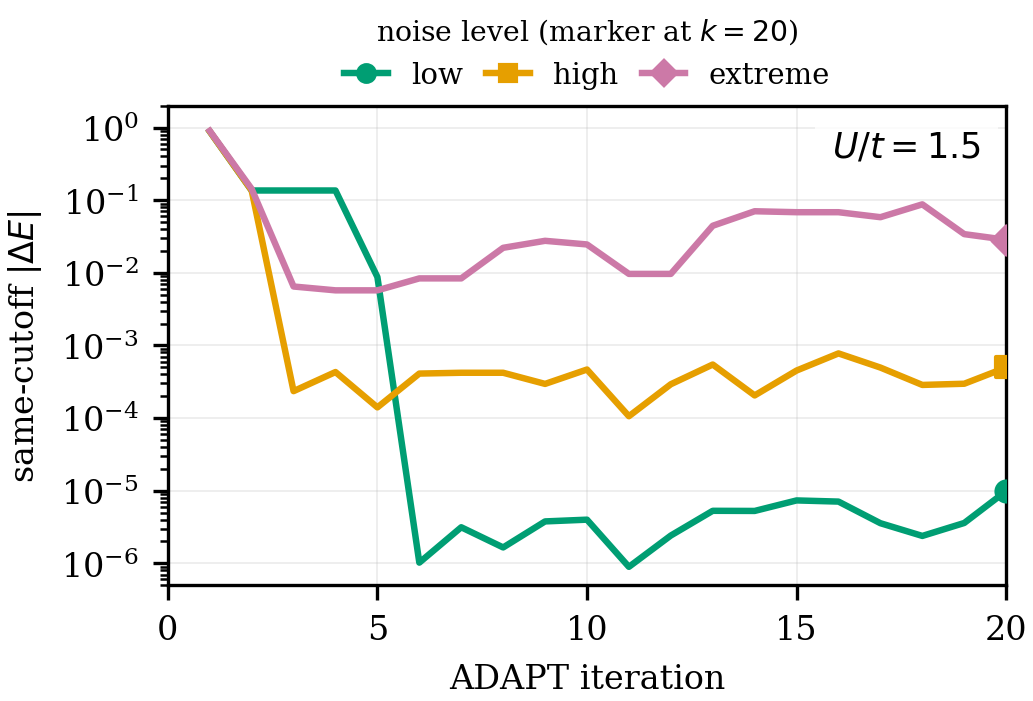
\includegraphics[width=0.475\textwidth]{figures/paper_i_hubbard_noise_common_prefix_k20_20260814/paper_i_hubbard_noise_u1p5_common_prefix_k20_20260814}
\hfill
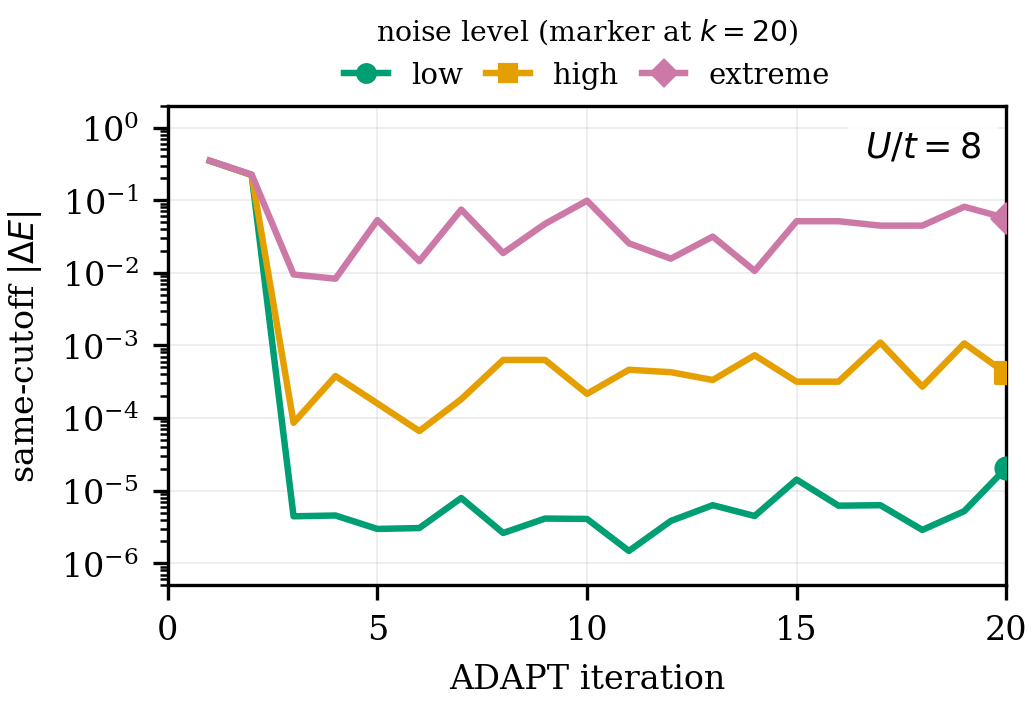
\includegraphics[width=0.475\textwidth]{figures/paper_i_hubbard_noise_common_prefix_k20_20260814/paper_i_hubbard_noise_u8_common_prefix_k20_20260814}
\caption{Same-cutoff energy error under simultaneous scalar value noise,
synthetic depolarizing gate noise, and frozen coherent overrotation noise for
the two-site Hubbard model at \(U/t=1.5\) (left) and \(U/t=8\) (right).
Low, high, and extreme denote the noise tuples in
Table~\ref{tab:hubbard_noise_levels}.  Every curve is displayed through the
common prefix \(k=20\); the single marker on each curve denotes that displayed
endpoint.}
\label{fig:hubbard_full_noise_common_prefix_k20}
\end{figure*}

% PROVENANCE(MACHINE_READABLE_HUBBARD_FULL_NOISE_COMMON_PREFIX_K20_20260814): {"display_k_max":20,"extreme_source_horizon":50,"figure_provenance":"MATH/paper_details/figures/paper_i_hubbard_noise_common_prefix_k20_20260814/paper_i_hubbard_noise_common_prefix_k20_20260814_provenance.json","figure_provenance_canonical_sha256":"db35df4c8f6976913645c858c2214cce6ea04dc944d4f6706e6da42359aa95be","figure_provenance_sha256":"ab4fb9643144a77d40c5242f1f7a20683d6b8e9b8b9c9167898fc9fc7c52c511","resource_ranges_exact":{"D2q":[28,109],"Dc":[287,797],"N2q":[38,136],"S_alg":[18286,96518],"W1q":[108,332]},"source_adapter":"output/pdf/paper_i_ra_adapt_stationary_core_full48_r50_20260728_evolving/paper_i_ra_adapt_stationary_core_full48_r50_20260728_evolving_pure_hubbard_page12_fullnoise_page15_adapter.json","source_adapter_canonical_sha256":"4991d37aa5c02d1cbd64ed5e707cd6e5265fed0563ad7c8b9c7b9d1f19439592","source_adapter_sha256":"92e0c559b82ca64ac5a4321f07e13a4433ee57e808eef76856da6051b207fa05"}

\clearpage
\begin{thebibliography}{99}

\bibitem{Hubbard1963}
J. Hubbard,
``Electron correlations in narrow energy bands,''
\emph{Proceedings of the Royal Society of London A} \textbf{276}, 238 (1963).

\bibitem{Holstein1959a}
T. Holstein,
``Studies of polaron motion: Part I. The molecular-crystal model,''
\emph{Annals of Physics} \textbf{8}, 325 (1959).

\bibitem{Holstein1959b}
T. Holstein,
``Studies of polaron motion: Part II. The small polaron,''
\emph{Annals of Physics} \textbf{8}, 343 (1959).

\bibitem{Sakkinen2015HolsteinDimer}
N. S\"akkinen, Y. Peng, H. Appel, and R. van Leeuwen,
``Many-body Green's function theory for electron-phonon interactions: Ground state properties of the Holstein dimer,''
\emph{Journal of Chemical Physics} \textbf{143}, 234101 (2015).

\bibitem{ClayHardikar2005HH}
R.~T. Clay and R.~P. Hardikar,
``Intermediate phase of the one-dimensional half-filled Hubbard-Holstein model,''
\emph{Physical Review Letters} \textbf{95}, 096401 (2005).

\bibitem{Tezuka2007HH}
A. Tezuka, R. Arita, and H. Aoki,
``Phase diagram for the one-dimensional Hubbard-Holstein model: a density-matrix renormalization group study,''
\emph{Physical Review B} \textbf{76}, 155114 (2007).

\bibitem{Weisse2008}
A. Wei{\ss}e and H. Fehske,
``Exact diagonalization techniques,''
in \emph{Computational Many-Particle Physics},
edited by H. Fehske, R. Schneider, and A. Wei{\ss}e,
Lecture Notes in Physics Vol. 739 (Springer, Berlin, Heidelberg, 2008), pp. 529--544.

\bibitem{Lloyd1996}
S. Lloyd,
``Universal quantum simulators,''
\emph{Science} \textbf{273}, 1073--1078 (1996).

\bibitem{AspuruGuzik2005}
A. Aspuru-Guzik, A.~D. Dutoi, P.~J. Love, and M. Head-Gordon,
``Simulated quantum computation of molecular energies,''
\emph{Science} \textbf{309}, 1704--1707 (2005).

\bibitem{Preskill2018NISQ}
J. Preskill,
``Quantum computing in the NISQ era and beyond,''
\emph{Quantum} \textbf{2}, 79 (2018).

\bibitem{Huggins2021Measurements}
W.~J. Huggins, J.~R. McClean, N.~C. Rubin, Z. Jiang, N. Wiebe, K.~B. Whaley, and R. Babbush,
``Efficient and noise resilient measurements for quantum chemistry on near-term quantum computers,''
\emph{npj Quantum Information} \textbf{7}, 23 (2021).

\bibitem{Romero2018UCC}
J. Romero, R. Babbush, J.~R. McClean, C. Hempel, P.~J. Love, and A. Aspuru-Guzik,
``Strategies for quantum computing molecular energies using the unitary coupled cluster ansatz,''
\emph{Quantum Science and Technology} \textbf{4}, 014008 (2018).

\bibitem{Peruzzo2014}
A. Peruzzo, J. McClean, P. Shadbolt, M.-H. Yung, X.-Q. Zhou, P.~J. Love, A. Aspuru-Guzik, and J.~L. O'Brien,
``A variational eigenvalue solver on a photonic quantum processor,''
\emph{Nature Communications} \textbf{5}, 4213 (2014).

\bibitem{McClean2016}
J.~R. McClean, J. Romero, R. Babbush, and A. Aspuru-Guzik,
``The theory of variational hybrid quantum-classical algorithms,''
\emph{New Journal of Physics} \textbf{18}, 023023 (2016).

\bibitem{Kandala2017}
A. Kandala, A. Mezzacapo, K. Temme, M. Takita, M. Brink, J.~M. Chow, and J.~M. Gambetta,
``Hardware-efficient variational quantum eigensolver for small molecules and quantum magnets,''
\emph{Nature} \textbf{549}, 242 (2017).

\bibitem{Cerezo2021VQA}
M. Cerezo, A. Arrasmith, R. Babbush, S.~C. Benjamin, S. Endo, K. Fujii, J.~R. McClean, K. Mitarai, X. Yuan, L. Cincio, and P.~J. Coles,
``Variational quantum algorithms,''
\emph{Nature Reviews Physics} \textbf{3}, 625--644 (2021).

\bibitem{VanStraaten2021MeasurementCost}
B. van Straaten and B. Koczor,
``Measurement cost of metric-aware variational quantum algorithms,''
\emph{PRX Quantum} \textbf{2}, 030324 (2021).

\bibitem{Grimsley2019}
H.~R. Grimsley, S.~E. Economou, E. Barnes, and N.~J. Mayhall,
``An adaptive variational algorithm for exact molecular simulations on a quantum computer,''
\emph{Nature Communications} \textbf{10}, 3007 (2019).

\bibitem{Grimsley2023ADAPT}
H.~R. Grimsley, G.~S. Barron, E. Barnes, S.~E. Economou, and N.~J. Mayhall,
``Adaptive, problem-tailored variational quantum eigensolver mitigates rough parameter landscapes and barren plateaus,''
\emph{npj Quantum Information} \textbf{9}, 19 (2023).

\bibitem{Tang2021}
H.~L. Tang, V.~O. Shkolnikov, G.~S. Barron, H.~R. Grimsley, N.~J. Mayhall, E. Barnes, and S.~E. Economou,
``Qubit-ADAPT-VQE: An adaptive algorithm for constructing hardware-efficient ans\"atze on a quantum processor,''
\emph{PRX Quantum} \textbf{2}, 020310 (2021).

\bibitem{Yordanov2021}
Y.~S. Yordanov, V. Armaos, C.~H.~W. Barnes, and D.~R.~M. Arvidsson-Shukur,
``Qubit-excitation-based adaptive variational quantum eigensolver,''
\emph{Communications Physics} \textbf{4}, 228 (2021).

\bibitem{Feniou2023}
C. Feniou, M. Hassan, D. Traor\'e, E. Giner, Y. Maday, and J.-P. Piquemal,
``Overlap-ADAPT-VQE: Practical quantum chemistry on quantum computers via overlap-guided compact ans\"atze,''
\emph{Communications Physics} \textbf{6}, 192 (2023).

\bibitem{Majland2024vADAPT}
M. Majland, P. Ettenhuber, N.~T. Zinner, and O. Christiansen,
``Vibrational ADAPT-VQE: Critical points lead to problematic convergence,''
\emph{Journal of Chemical Physics} \textbf{160}, 154109 (2024).

\bibitem{Athanasakos2026CVADAPT}
D. Athanasakos, G. Tejedor-Garc\'ia, J.~Y. Araz, M. Ram\^oa, B. Sambasivam, S.~E. Economou, and F. Ringer,
``Continuous-variable ADAPT-VQE for bosonic lattice models,''
\emph{arXiv:2606.05297} (2026).

\bibitem{Anastasiou2024}
P.~G. Anastasiou, Y. Chen, N.~J. Mayhall, E. Barnes, and S.~E. Economou,
``TETRIS-ADAPT-VQE: An adaptive algorithm that yields shallower, denser circuit ans\"atze,''
\emph{Physical Review Research} \textbf{6}, 013254 (2024).

\bibitem{Ramoa2025}
M. Ram\^oa, P.~G. Anastasiou, L.~P. Santos, N.~J. Mayhall, E. Barnes, and S.~E. Economou,
``Reducing the resources required by ADAPT-VQE using coupled exchange operators and improved subroutines,''
\emph{npj Quantum Information} \textbf{11}, 86 (2025).

\bibitem{Ramoa2025HessianRecycling}
M. Ramoa et al.,
``Reducing measurement costs by recycling the Hessian in adaptive variational quantum algorithms,''
\emph{Quantum Science and Technology} \textbf{10}, 015031 (2025).

\bibitem{He2026ParamADAPT}
R. He, X. Hong, Q. Chai, J. Guan, J. Zhou, A. Ablimit, G. Cui, and S. Ying,
``Constructing Compact ADAPT Unitary Coupled-Cluster Ansatz with Parameter-Based Criterion,''
\emph{Journal of Chemical Theory and Computation} \textbf{22}, 5090--5101 (2026).

\bibitem{He2026HAADAPT}
R. He, C. Liu, X. Hong, Q. Chai, J. Zhou, J. Guan, G. Cui, and S. Ying,
``Hamiltonian-Aware ADAPT Variational Quantum Eigensolver for Molecular Ground-State Simulation,''
\emph{arXiv:2606.13118} (2026).

\bibitem{Bespalova2026KADAPT}
T.~A. Bespalova, O. Ladhari, and G. Masella,
``K-ADAPT-VQE: Optimizing Molecular Ground State Searches by Chunking Operators,''
in \emph{Quantum Engineering Sciences and Technologies for Industry and Services}, Communications in Computer and Information Science \textbf{2744}, 226--235 (Springer, Cham, 2026).

\bibitem{Nocedal2006TrustRegion}
J. Nocedal and S. J. Wright,
\emph{Numerical Optimization}, 2nd ed.
(Springer, New York, 2006).

\bibitem{IglewiczHoaglin1993}
B. Iglewicz and D.~C. Hoaglin,
\emph{How to Detect and Handle Outliers},
ASQC Basic References in Quality Control: Statistical Techniques, Vol.~16
(ASQC Quality Press, Milwaukee, WI, 1993).

\bibitem{Ikhtiarudin2025ShotEfficient}
A. Ikhtiarudin, G. K. Sunnardianto, F. Fathurrahman, M. K. Agusta, and H. Dipojono,
``Shot-Efficient ADAPT-VQE via Reused Pauli Measurements and Variance-Based Shot Allocation,''
\emph{arXiv:2507.16879} (2025).

\bibitem{Lowerre1976Beam}
B. T. Lowerre,
``The Harpy Speech Recognition System,''
Ph.D. thesis, Carnegie Mellon University (1976).

\bibitem{Sohail2026GeoADAPT}
M.~A. Sohail and T. Koike-Akino,
``Geo-ADAPT-VQE: Quantum Information Metric-Aware Circuit Optimization for Quantum Chemistry,''
\emph{arXiv:2603.10325} (2026).

\bibitem{Stadelmann2025GradientTroughs}
T. Stadelmann and others,
``Strategies for overcoming gradient troughs in the ADAPT-VQE algorithm,''
\emph{arXiv:2512.25004} (2025).

\bibitem{ProvostVallee1980}
J.-P. Provost and G. Vall\'ee,
``Riemannian structure on manifolds of quantum states,''
\emph{Communications in Mathematical Physics} \textbf{76}, 289 (1980).

\bibitem{Stokes2020QNG}
J. Stokes, J. Izaac, N. Killoran, and G. Carleo,
``Quantum natural gradient,''
\emph{Quantum} \textbf{4}, 269 (2020).

\bibitem{Haug2021Capacity}
T. Haug, K. Bharti, and M.~S. Kim,
``Capacity and quantum geometry of parametrized quantum circuits,''
\emph{PRX Quantum} \textbf{2}, 040309 (2021).

\bibitem{JavadiAbhari2024Qiskit}
A. Javadi-Abhari, M. Treinish, K. Krsulich, C.~J. Wood, J. Lishman, J. Gacon, S. Martiel, P.~D. Nation, L.~S. Bishop, A.~W. Cross, B.~R. Johnson, and J.~M. Gambetta,
``Quantum computing with Qiskit,''
\emph{arXiv:2405.08810} (2024).

\bibitem{QiskitAlgorithmsAdaptVQE}
Qiskit Community,
``AdaptVQE,''
\emph{Qiskit Algorithms 0.4.0 documentation},
\url{https://qiskit-community.github.io/qiskit-algorithms/stubs/qiskit_algorithms.AdaptVQE.html}
(accessed July 27, 2026).

\bibitem{Verteletskyi2020CliqueCover}
V. Verteletskyi, T.-C. Yen, and A.~F. Izmaylov,
``Measurement optimization in the variational quantum eigensolver using a minimum clique cover,''
\emph{Journal of Chemical Physics} \textbf{152}, 124114 (2020).

\bibitem{Yen2020CompatibleMeasurements}
T.-C. Yen, V. Verteletskyi, and A.~F. Izmaylov,
``Measuring all compatible operators in one series of single-qubit measurements using unitary transformations,''
\emph{Journal of Chemical Theory and Computation} \textbf{16}, 2400 (2020).


\bibitem{Macridin2018}
A. Macridin, P. Spentzouris, J. Amundson, and R. Harnik,
``Electron-phonon systems on a universal quantum computer,''
\emph{Physical Review Letters} \textbf{121}, 110504 (2018).

\bibitem{Sawaya2020}
N.~P.~D. Sawaya, T. Menke, T.~H. Kyaw, S. Johri, A. Aspuru-Guzik, and G.~G. Guerreschi,
``Resource-efficient digital quantum simulation of $d$-level systems for photonic, vibrational, and spin-$s$ Hamiltonians,''
\emph{npj Quantum Information} \textbf{6}, 49 (2020).

\bibitem{Li2023}
W. Li, J. Ren, S. Huai, T. Cai, Z. Shuai, and S. Zhang,
``Efficient quantum simulation of electron-phonon systems by variational basis state encoder,''
\emph{Physical Review Research} \textbf{5}, 023046 (2023).

\bibitem{Denner2023}
M.~M. Denner, A. Miessen, H. Yan, I. Tavernelli, T. Neupert, E. Demler, and Y. Wang,
``A hybrid quantum-classical method for electron-phonon systems,''
\emph{Communications Physics} \textbf{6}, 233 (2023).

\bibitem{Peng2025BosonHamiltonians}
B. Peng, Y. Su, D. Claudino, K. Kowalski, G. H. Low, and M. Roetteler,
``Quantum simulation of boson-related Hamiltonians: Techniques, effective Hamiltonian construction, and error analysis,''
\emph{Quantum Science and Technology} \textbf{10}, 023002 (2025).

\bibitem{Vaquero2025PrunedADAPT}
N. Vaquero-Sabater, A. Carreras, and D. Casanova,
``Pruned-ADAPT-VQE: Compacting Molecular Ans\"atze by Removing Irrelevant Operators,''
\emph{Journal of Chemical Theory and Computation} \textbf{21}, 8720--8728 (2025).

\end{thebibliography}

\end{document}
